The final design can be segmented into 2 stages: the data acquisition unit and the machine learning unit. Connecting these two parts of the project is the data refinement process. In a broad overview, the data generated by either the heating chamber or the MATLAB simulation were processed and input into the Random Forests and LSTM neural network. Each component of this is detailed below.

\subsection{Data Acquisition}
The data acquisition unit consists of the curing oven, the PID control system, the temperature sensors that provide the temperature data, and the microcontroller that reads and logs the data. The curing oven and PID control system remain unchanged from their initial setup. %Due to the premature closure of the lab, no photographs of the setup were taken, as all equipment was left in the lab.

\subsubsection{Curing Oven Configuration}
The curing oven configuration consisted of four 100k NTC thermistors for recording the external air temperature around a test object with an internal thermistor. The object used in the experiment was an aluminum cylinder of 3 cm radius, and 5 cm height. A hole was drilled into the cylinder with a depth of 2.5 cm in which we inserted a thermistor. The metal cylinder was held by a raised 10cm wooden platform with studded ends. This was to keep the cylinder isolated from other heat sinks. A mockup of the design is shown in Figure \ref{fig:heat_chamber_cad} with the heat source in red, the cylinder in white, and the thermistors connected to the black wires. 

\subsubsection{Temperature Sensor Configuration}
The three external thermistors were placed close to the surface of the cylinder. They were positioned above, below, and on the side of the cylinder. It was found that due to constant temperature on the horizontal plane, any extra thermistors would unnecessarily increase the amount of data. While three thermistors were used, due to the vertical temperature gradient of the heat chamber, the central side thermistor was weighted higher than the other two for determining the average external temperature as it was reflective of the mean temperature due to symmetry.
\newpage
\begin{figure}[!htb]
    \centering
    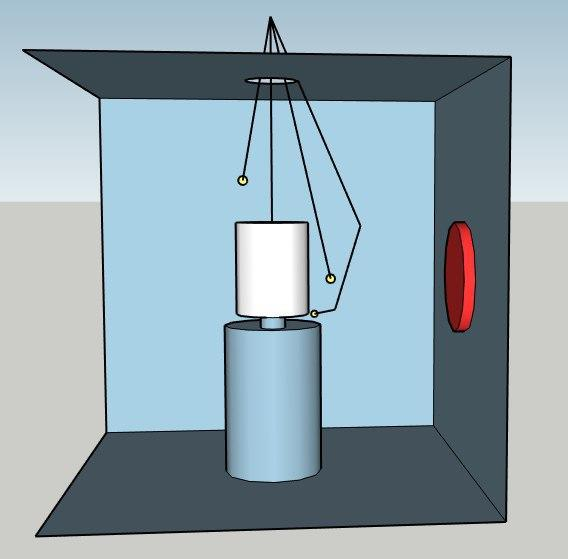
\includegraphics[width=0.4\linewidth, frame]{other/heat_chamber_cad.jpg}
    \caption{CAD Drawing of Heat Chamber Test Configuration}
    \label{fig:heat_chamber_cad}
\end{figure}
\subsubsection{Microcontroller Configuration}
The data we collected was collected on the TM4C123G. Our preliminary design initially developed consisted of thermistors connected to a Texas Instruments TM4C123G. To increase accuracy and computational power we changed our data acquisition unit to a Raspberry Pi 4 with an external ADC used to interface the thermistors to the Raspberry Pi. The ADC is connected to the midpoint of a voltage divider between the thermistor and a 100k $\Omega$ resistor. Steinhart-Hart equations shown below as Equation \ref{shheq1} \& \ref{shheq2} were used to covert the voltage reading to a temperature reading, using coefficients found from \cite{shheq} and the table \cite{ttable} containing resistance values for our thermistors along.    
\begin{equation} \label{shheq1}
    R_{thermistor} = \frac{100k \Omega}{ V_{dc} / (V_{dc} - V_{adc reading}) - 1.0}
\end{equation}
\begin{align*}
Where \\
c1 = 0.6764629190e-03 \\
c2 = 2.230798167e-04 \\
c3 = 0.7159342899e-07
\end{align*}
\begin{equation} \label{shheq2}
    \text{Temperature In Celsius} = \frac{1.0}{c1 + c2 * ln(R_{thermistor}) + c3 * ln(R_{thermistor})^3)} - 273.15
\end{equation}
% The advantages of using this system aside from more accurate temperature readings are that the Raspberry Pi has more computational capability compared to the TM4C123G. This additional computational ability allows for the potential to train a machine learning model on the data acquisition unit itself. Alternatively, an already trained model can potentially be loaded onto the Raspberry Pi and incoming data can be fed through the machine learning model for live prediction. In addition, the Raspberry Pi has wireless internet capability built in, allowing for potential integration with cloud storage and/or computation services. Due to the abrupt and unexpected inability to access the lab as of March 16, we were unable to collect data using the new Raspberry Pi based data acquisition unit.

\subsubsection{Obtained Data}
Through three separate runs, the following data was collected. The runs were collected using multiple air temperature sensors and a single sensor for the part temperature. The air temperature exhibits a very steep rise and some overshoot then a gradual rise towards zero error. The part temperature shows a initial steep rise which is believed to be caused by a large amount infrared radiation from the lamp being on for high duty cycles. After the initial rise, the duty cycle becomes more normalized to about 30\% and the rise is uniform. The end of the runs are not fully converged and usually stop before they are completely equal but for runs 1 and 2 they are within 5\% tolerance. The runs also have a Gaussian noise in the readings due to variance in the electronic ADC reading, and fluctuations in air temperature.
\begin{figure}[ht]
    \begin{subfigure}{.33\linewidth}
        \centering
    	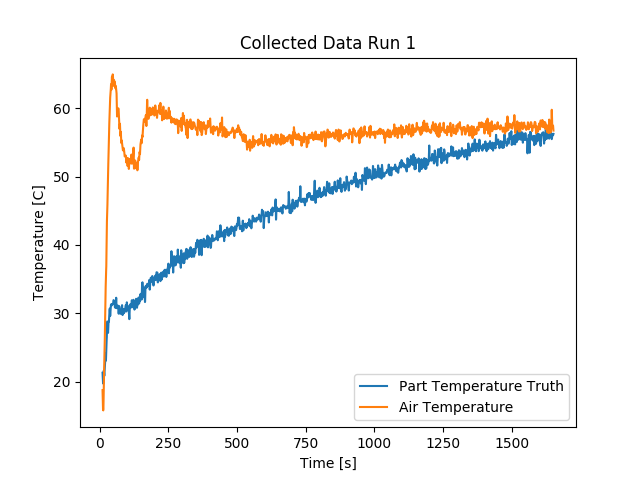
\includegraphics[width=\linewidth]{other/Raw_Data/1.png}
        \caption{Run 1}
    \end{subfigure}
    \begin{subfigure}{.33\linewidth}
        \centering
    	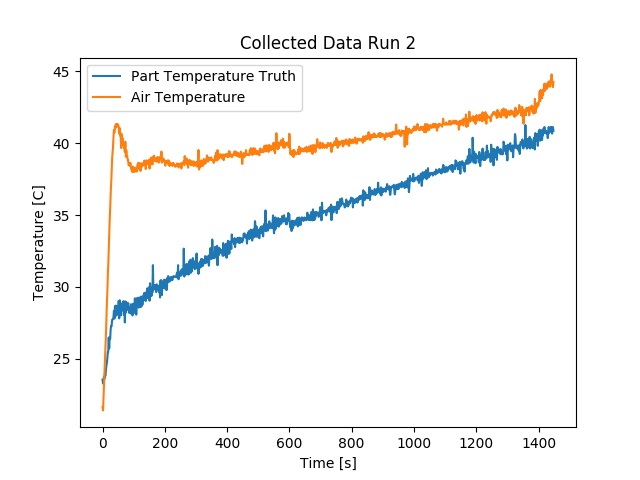
\includegraphics[width=\linewidth]{other/Raw_Data/2.png}
    	\caption{Run 2}
    \end{subfigure}
    \begin{subfigure}{.33\linewidth}
        \centering
    	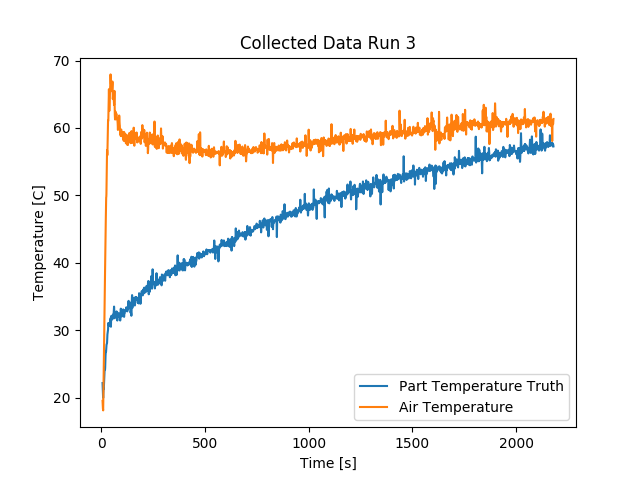
\includegraphics[width=\linewidth]{other/Raw_Data/3.png}
    	\caption{Run 3}
    \end{subfigure}\par\medskip
    \caption{Data Collected from Runs 1 to 3}
    \label{fig:real_data0-3}
\end{figure}

\subsection{MATLAB Data Generation}
Here the methods for creating the MATLAB transient heat simulations for this project are explained and their results are examined. The general methodology used for generating these simulations are discussed. The specific toolboxes, functions, and strategies implemented in MATLAB are then described in this section. \\\\
The purpose of generating transient heat simulations is so the resulting data can be used for testing and training our machine learning models. Through research and investigation we found that MATLAB could be implemented for generating data sets using its finite element analysis features for modelling heat transfer problems. Building these heat simulations also made it feasible to study different materials, geometries, and temperature distributions. 

\subsubsection{Governing Equations}
For our transient heat simulations it was important to understand the governing equation that models the heat transfer problem. Using the approximation of a rectangular block revolved around the central axis, an idealized thermal equation was needed to create the simulations. Equation \ref{equation_matlab} shows the PDE used to model the transient conduction for the heat transfer problem. With T being temperature, $\rho$ is material density, $C_{p}$ is the specific heat value, $k$ is the thermal conductivity, and $f$ is the heat generated inside the cylinder. This equation is temperature dependent and is used to govern the heat conduction through the cylinder. 
\begin{equation}
    \rho C_p \frac{dT}{dt}   - \nabla \cdot (k \nabla T) = f 
    \label{equation_matlab}
\end{equation}

\subsubsection{MATLAB Simulated Data Generation}
First, using the \lstinline{createpde} function a PDE model of the system is created and it also sets up a transient simulation on this PDE model. Next, the geometry of the cylinder and the surrounding shape of the air is programmed. The geometry of the cylinder was approximated by using a 2D rectangle and revolving it around its central axis would then create a cylinder. This geometry is enclosed with boundary conditions set to represent the surrounding air inside the heating chamber. In Figure \ref{fig:matlab_heatchamber} this model is plotted showing the cylinder and the surrounding air with their position along the X and Y axes. This model also has the thermal properties programmed for the air and aluminum cylinder so the thermal conductivity across the cylinder can then be simulated. Then the temperature conditions were set to heat from the boundaries or edges ‘E1, E2, E6, E7’ of Figure \ref{fig:matlab_heatchamber} which gave a realistic simulation of the infrared lamp heating the cylinder from all directions. The \lstinline{transientBCHeatedBlock} function was used to set the initial, rise, and final temperatures on these edges. This function allowed us to set the temperature conditions for the simulation to mimic the curing cycles in the physical heating chamber experiments as accurately as possible.
\begin{figure}[!htb]
    \begin{subfigure}{.5\linewidth}.
        \centering
        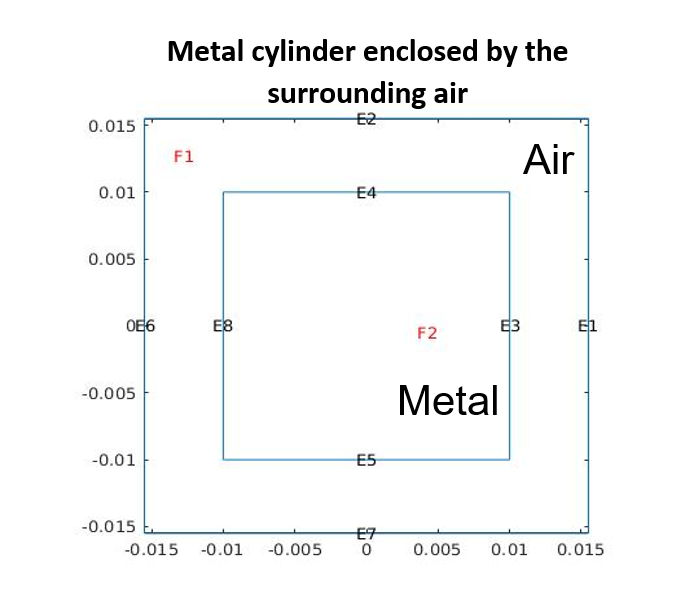
\includegraphics[width=0.65\linewidth]{other/metal_cylinder_mesh.png}
        \caption{Mesh of Metal Cylinder Approximation}
        \label{fig:matlab_heatchamber}
    \end{subfigure}
    \begin{subfigure}{.5\linewidth}.
        \centering
        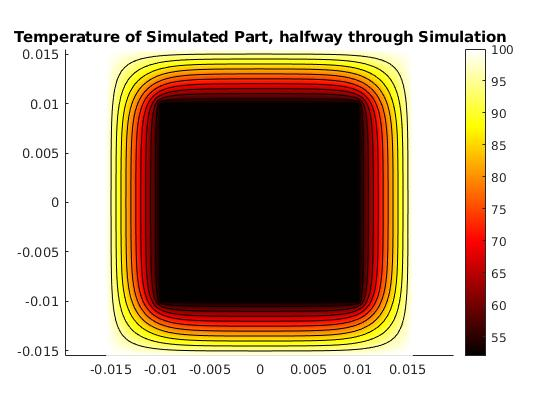
\includegraphics[width=0.7\linewidth]{other/transient_solution.png}
        \caption{Heat Distribution from Simulation}
        \label{fig:transient_solution}
    \end{subfigure}
    \caption{Heat Chamber Simulations using MATLAB}
\end{figure}

Having the model geometry, material properties, and boundary conditions symmetrical about the central axis also created a uniform heat distribution across the simulated cylinder. %It was known from experimental testing that the center of the cylinder heated up slower than the outer surface due to the aluminum’s thermal conductivity.
For the simulations a PDE with constant thermal conductivity and material properties not temperature dependent were assumed. %This was based on experimental observations of the conductive heat transfer through the material. The assumption is seen in the MATLAB script with the thermal conductivity value being set as a constant throughout the simulation. 
Combining the external air temperature conditions with this constant thermal conductivity assumption produced a representation of the cylinder’s internal temperature over time. 
The results from Figure \ref{fig:transient_solution} shows the simulation halfway through where there is a uniform heat distribution across the cylinder which is lagging behind the air temperature which is at 100$^\circ$C.

\subsubsection{Transient Heat Simulation Outputs}
The last part of these MATLAB simulations was to generate the transient response of the model and evaluate the outputs. This was easily done using more built-in functions in the PDE toolbox. In MATLAB, the simulations were programmed to capture the temperatures at the air boundary and the center of the cylinder. The simulation is also set to save the temperature data every 1 second over the entire heating cycle. Then when the code is run, multiple time series data sets are produced showing ideal curing cycles. An example of a simulated curing cycle generated with MATLAB is shown in Figure \ref{fig:comparison_sim_real}a with a maximum curing temperature of 85$^\circ$C. Then in Figure \ref{fig:comparison_sim_real}b the curing cycle of a real data set is shown with maximum temperature at 60$^\circ$C. The MATLAB data set shows the air temperature’s curve having a more gradual rise compared to the curve from the heat chamber data set. This due to the settings of the PID controller in the heat chamber programmed to ramp up faster than the simulation. However, the simulations still provide robust data for training machine learning algorithms which will be able to predict the heat chamber conditions when fed experimental data after being trained on these simulated data sets.\\\\
The MATLAB transient heat simulations satisfied their overall purpose of generating multiple data sets with varying parameters. It was possible to change parameters like shape, material, conductivity of air, and temperature conditions without doing time-consuming experimental runs in the laboratory. The MATLAB code also has the ability to perform the simulations with different parameters in parallel. The parallelization of the data generation code reduced the runtime for generating 20 data sets from 1.5 hours down to approximately 15 minutes. 

\begin{figure}[!htb]
    \begin{subfigure}{.5\linewidth}.
        \centering
    	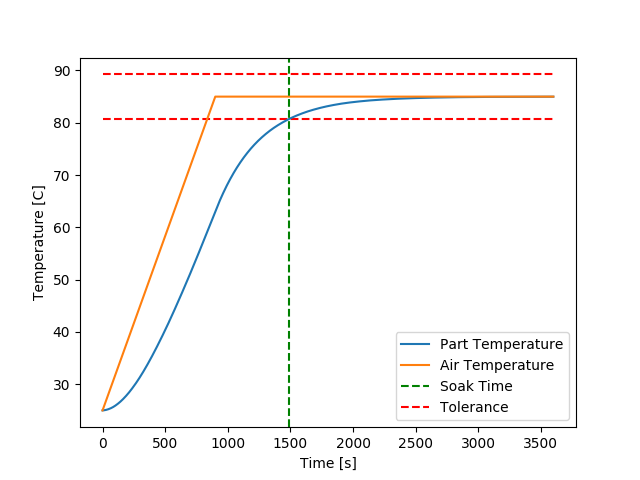
\includegraphics[width=0.9\linewidth]{other/sim_data.png}
        \caption{Simulated Data with a 5\% tolerance marked and soak time}
    \end{subfigure}
    \begin{subfigure}{.5\linewidth}.
        \centering
    	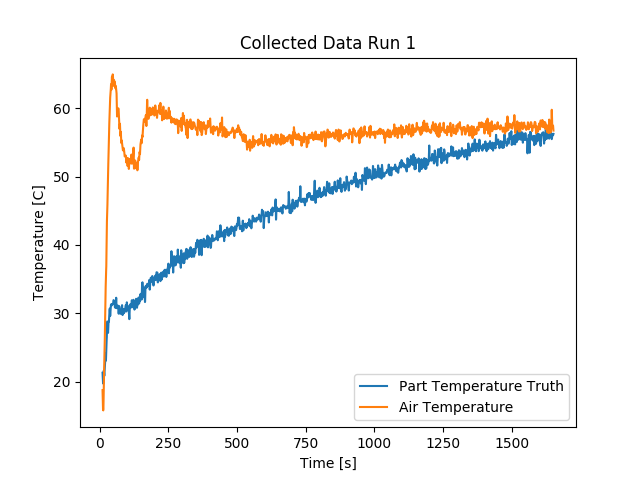
\includegraphics[width=0.9\linewidth]{other/Raw_Data/1.png}
        \caption{Curing Cycle using Real Dataset}
    \end{subfigure}
    \caption{Comparison of Simulations and Real Data}
	\label{fig:comparison_sim_real}
\end{figure}
\clearpage

\subsection{Data Filtering}
In this project, it was in our interest to understand the effects of noise from our temperature sensors on the machine learning process. We wanted to know if noise from the sensors was affecting the soak time estimate and if noise would affect the accuracy of the prediction by the machine learning methods, as the data to train on would be more inconsistent with noise present. To perform our analysis, we began by running our data through various filters: A Savitzky-Golay filter and a Kalman filter, both implemented in Python. A Savitzky-Golay filter was chosen because it is an effective filter for smoothing data through local regression and can be implemented with ease. The Savitzky-Golay filter is more sensitive to bursts of noise and therefore has the possibility of skewing the signal, however it seemed like an appropriate fit due to the uniformity of our data. A comparison of the filtered data using Savitzky-Golay filter and the unfiltered data can be seen in Figure \ref{fig:savitzky} below. It can be observed that despite some inaccuracy located after the initial rise in temperature, the filter was effective in smoothing the data. Following this, we ran our sample data through a Kalman filter. For our application, the Kalman filter was used to extract the signal from the noise, which provided us with a significantly more accurate representation of the signal with smaller noise margins. The Kalman filtered data and the unfiltered data are compared in Figure \ref{fig:kalman}. The filter was ultimately able to fulfill our intended application.\\\\
To test our concerns, we trained our machine learning methods and performed predictions using unfiltered data, the Savitzky-Golay filtered data, and the Kalman filtered data. We then performed a comparative analysis on the soak time estimates of each prediction and the accuracy of each prediction relative to the true temperature of the cylinder. The figures below demonstrate the predictions from the aforementioned data through the LSTM method and the Random Forests method, respectively, for one sample run from our data set. From our analysis, we observed minor improvements through filtering the data with the Kalman filter, with similar albeit not as improved results using the Savitzky-Golay filter regarding the accuracy of the predictions. We did not observe any difference in the estimated soak time from filtering the data. We were ultimately able to conclude that the effects of noise are mostly negligible for the project application, as the noise did not have any significant impact on the machine learning process or the soak time. Further data analysis in this report is performed with the Kalman filtered data, as it provides a more visually informative and accurate view of the relationships between the curves in plotting.

\begin{figure}[h]
    \begin{subfigure}{.5\linewidth}.
        \centering
    	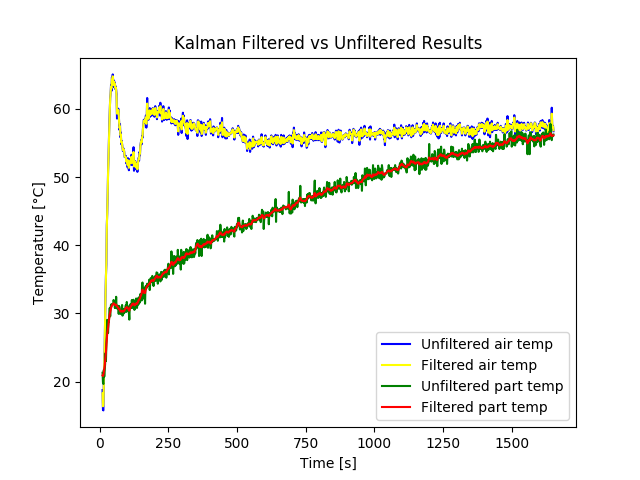
\includegraphics[width=1\linewidth]{filter/kalman.png}
        \caption{Kalman Filtered Data}
        \label{fig:kalman}
    \end{subfigure}
    \begin{subfigure}{.5\linewidth}.
        \centering
    	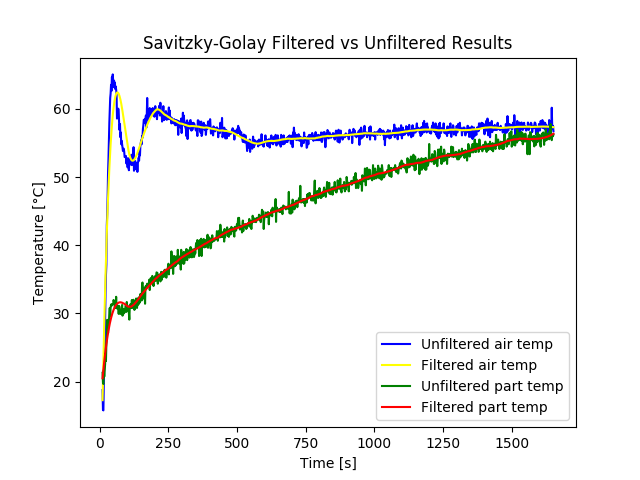
\includegraphics[width=1\linewidth]{filter/savitzky.png}
        \caption{Savitzky-Golay Filtered Data}
    	\label{fig:savitzky}
    \end{subfigure}
    \caption{Data Filtering Techniques}
\end{figure}
\begin{figure}[ht]
    \vspace{-0.9cm}
    \begin{subfigure}{.34\linewidth}.
        \centering
    	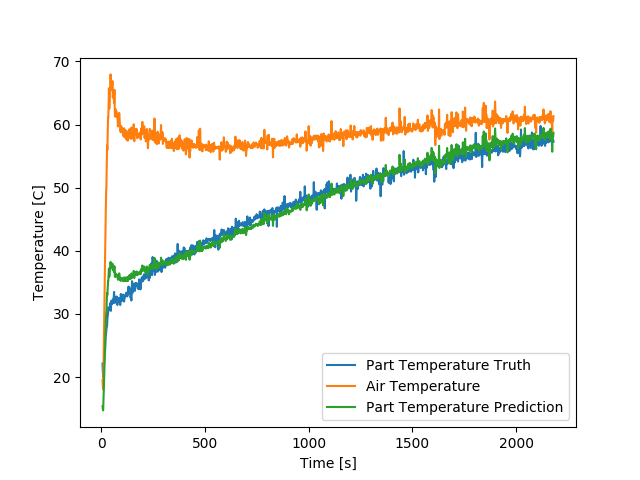
\includegraphics[width=1.1\linewidth]{filter/unfiltered_LSTM.png}
        \caption{Unfiltered Data with LSTM}
    \end{subfigure}
    \begin{subfigure}{.34\linewidth}
    	\centering
    	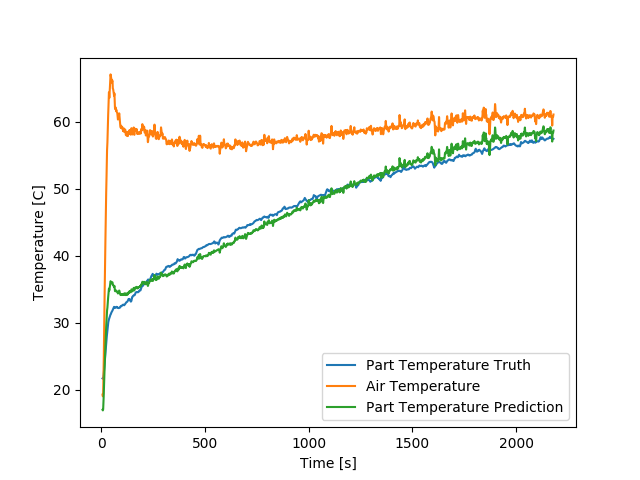
\includegraphics[width=1.1\linewidth]{filter/kalman_LSTM.png}
        \caption{Kalman Data with LSTM}
    \end{subfigure}
    \begin{subfigure}{.34\linewidth}
    	\centering
    	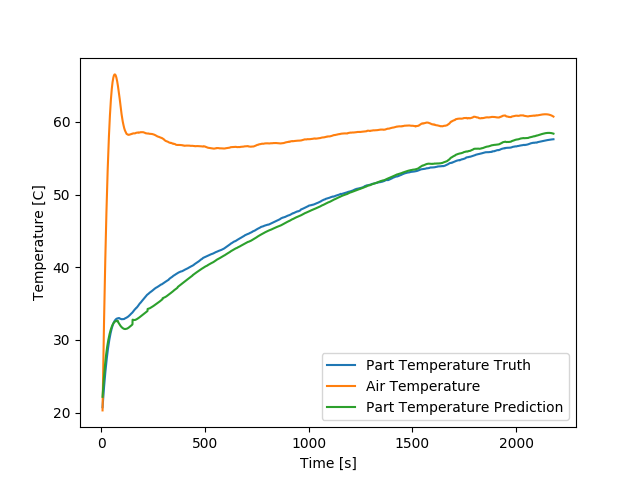
\includegraphics[width=1.1\linewidth]{filter/savitzky_prediction_LSTM.png}
    	\caption{Savitzky Data with LSTM}
    \end{subfigure}
    \caption{Predictions using Filtered Data with LSTM}
\end{figure}

\begin{figure}[ht]
    \begin{subfigure}{.34\linewidth}.
        \centering
    	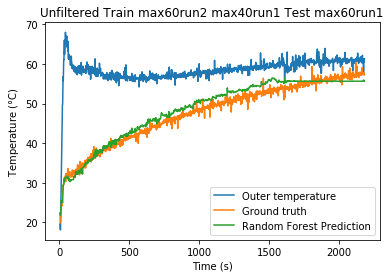
\includegraphics[width=\linewidth]{filter/unfiltered_RF.png}
        \caption{Unfiltered Data with Random Forest}
    \end{subfigure}
    \begin{subfigure}{.34\linewidth}
    	\centering
    	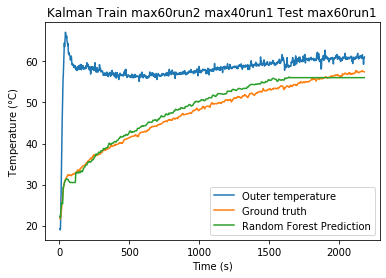
\includegraphics[width=\linewidth]{filter/kalman_RF.png}
        \caption{Kalman Data with Random Forest}
    \end{subfigure}
    \begin{subfigure}{.34\linewidth}
    	\centering
    	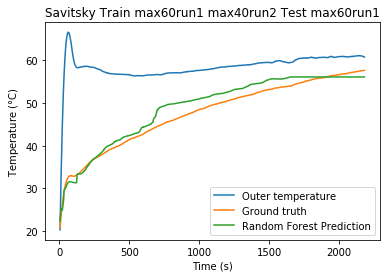
\includegraphics[width=\linewidth]{filter/savitzky_RF.png}
    	\caption{Savitzky Data with Random Forest}
    \end{subfigure}
    \caption{Predictions using Filtered Data with Random Forest}
\end{figure}\clearpage
\subsection{Data Scaling}
To input the data into a neural network, it improves performance to manipulate the data and scale it between values of 0 and 1. Large inputs which are disproportionate to each other can slow down the convergence of the training algorithm and can in some cases prevent the neural network from classifying the problem \cite{hands_on_scaling}. A \lstinline{min_max} function is used to scale the input data between ranges min and max, which are commonly set to values 0 and 1 respectively. 
\begin{equation} \label{scaled_eq1}
    X_{std} = \frac{(X - X_{min})}{(X_{max} - X_{min})}
\end{equation}
\begin{equation} \label{scaled_eq2} 
    X_{scaled} = X_{std} (max - min) + min
\end{equation}

Time, if desired as an input feature to the neural network, can be scaled from 0 to 1 signifying the duration of the run from  start to finish. As all runs follow a predictable start and finish, where at the start part temperature is equal to air temperature and at the end of the run the same is true. The time data can then be a feature which shows where in the run the network is, and if needed expanded beyond 1 to predict future data which has never been seen by the neural network. Temperature data can be scaled so the minimum temperature across all runs training runs is the minimum value used in equation \ref{scaled_eq2}, and the max temperature value across all training runs is the value used in  \ref{scaled_eq2}. The scaling is shown below in Figure \ref{fig:scale1}. It can be seen that the two runs which were set to 60$^\circ$C are similar in nature and the run which is set to 40$^\circ$C is obviously lower. Time is scaled from 0 to 1. All runs are interpolated to be the same size which is used for the LSTM network.\\
\begin{figure}[h]
    \centering
    \vspace{-25pt}
    \centerline{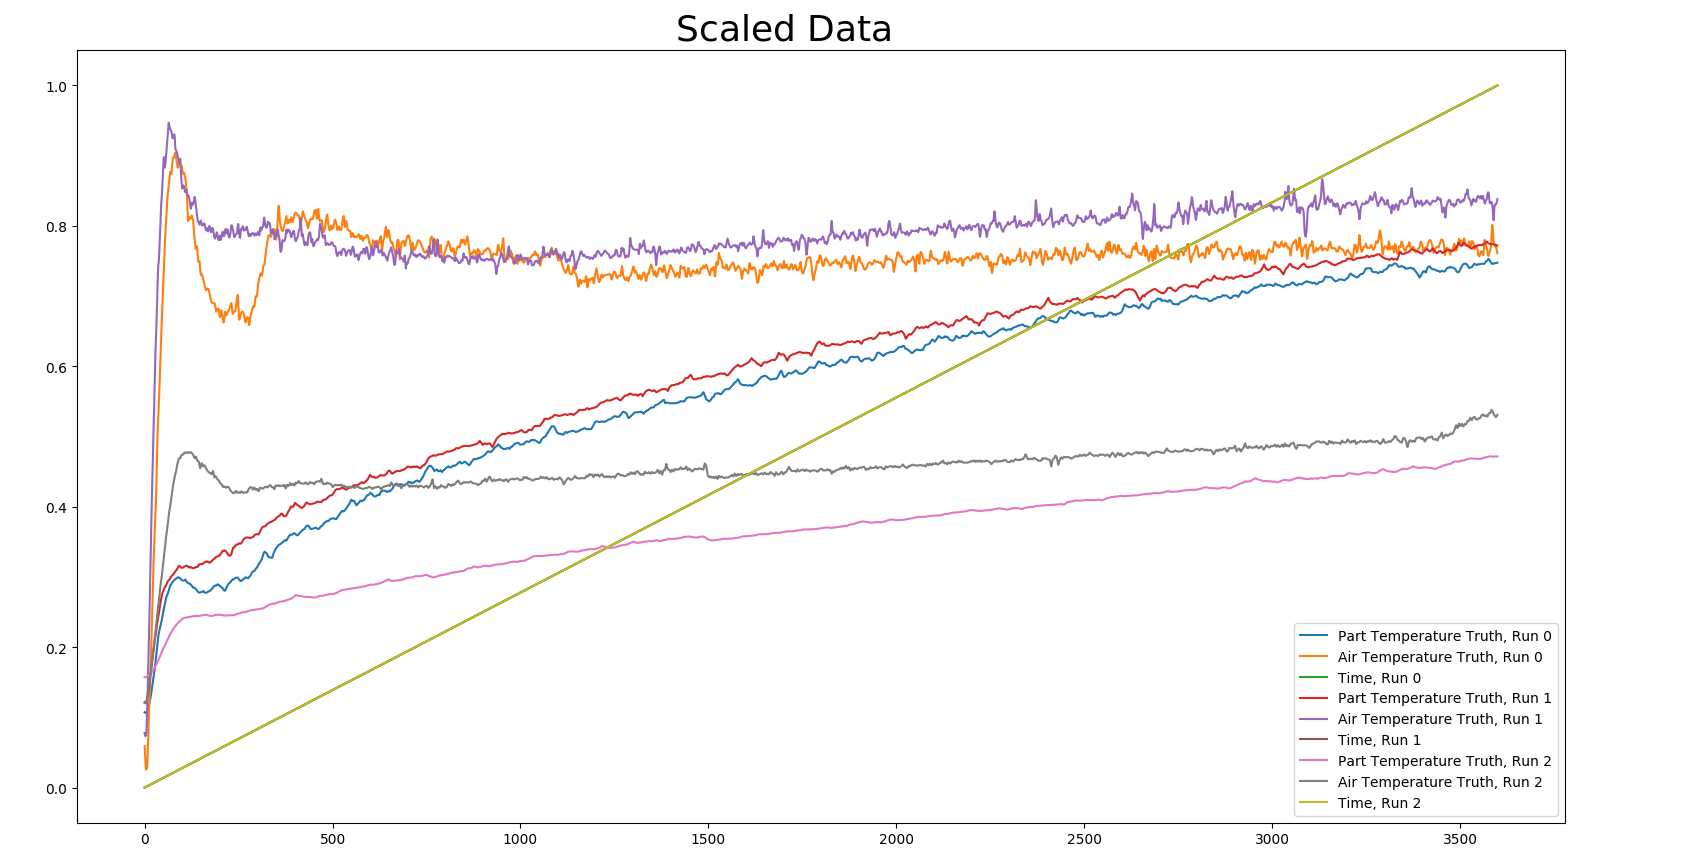
\includegraphics[width=0.9\linewidth]{scaling/image1.png}}
    \caption{Scaling Input Features Part and Air Temp, and Time using Predefined Constants for Temperatures}
    \label{fig:scale1}
\end{figure}
\newpage
%Alternatively, temperature can be scaled on a per run basis, meaning that the max and min are set per run and not as a max/min for all runs. The result is a series of similar curves which all follow the same slope and value profile which is shown below in Figure \ref{fig:scale2}. The main disadvantage is that this method loses the scale of the temperature and instead just shows how it changes during a run. In the end, this method produces greater error and was not used as the scaling lost essential data, as the neural network does not know that run 2 was the lowest temperature run which resulted in the part temperature rising the slowest. This method could be useful if temperature was not a feature that changed between runs or if time series temperature data itself held some kind of slope which implied a higher or lower temperature. This scaling might be used if one wanted to reduce training time and get a result which is more general.
%\begin{figure}[htb]
%    \centering
%    \centerline{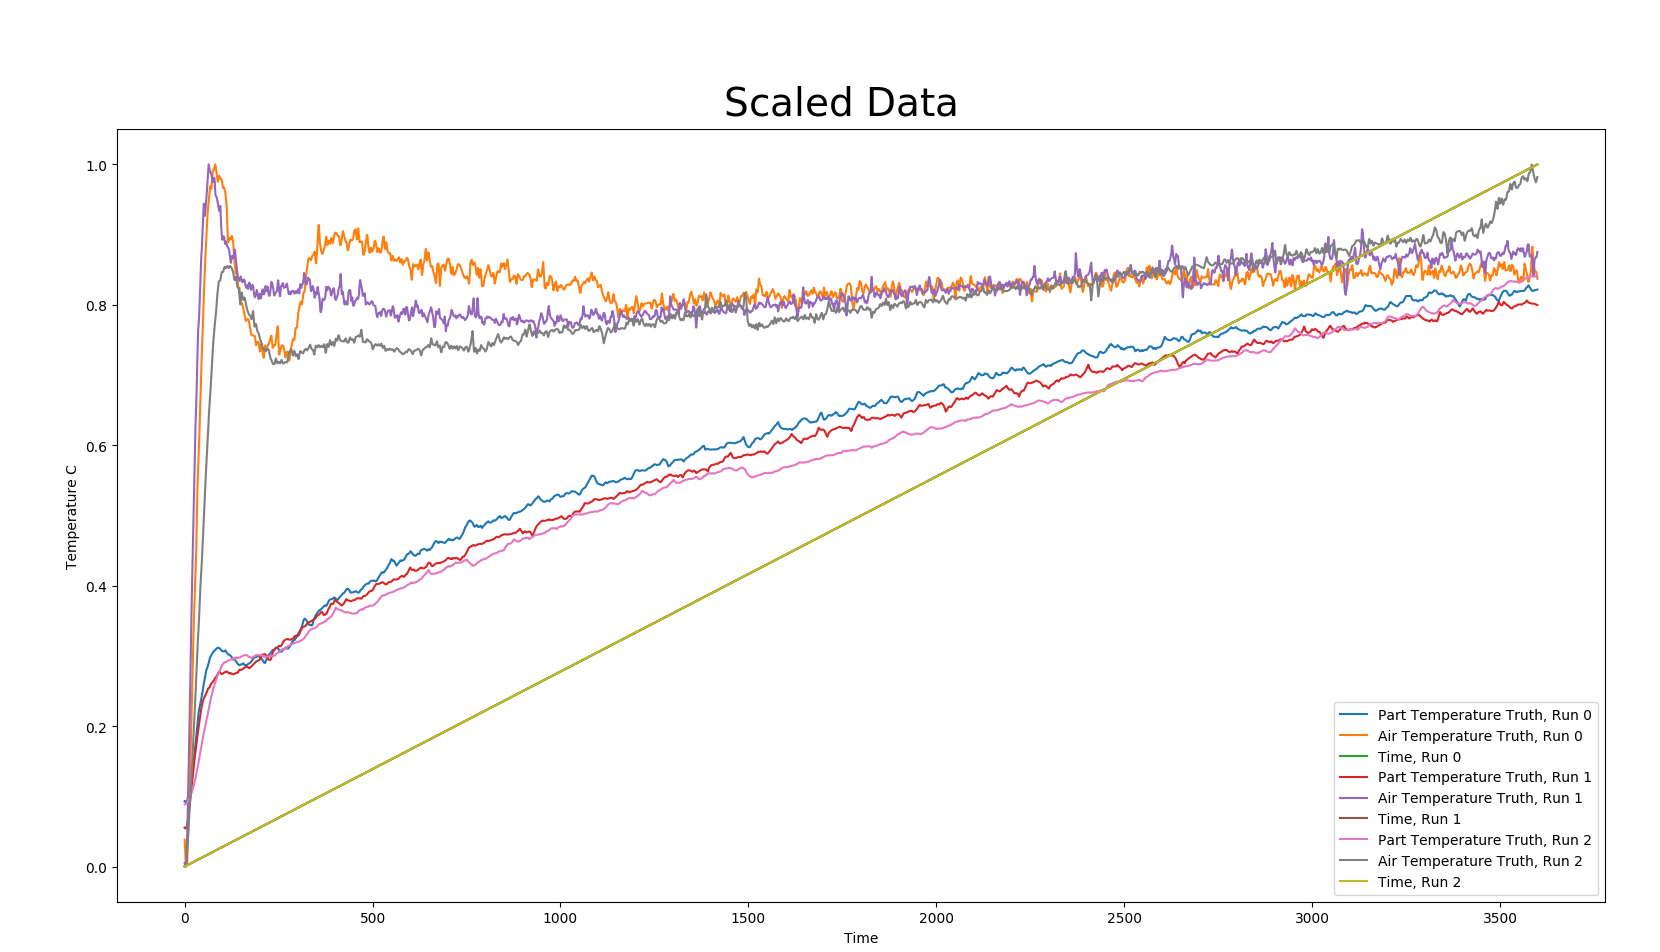
\includegraphics[width=0%.9\linewidth]{scaling/image12.png}}
%    \caption{Scaling Input Features %using Maximums and Minimums}
%    \label{fig:scale2}
%\end{figure}
\subsection{Recurrent Neural Networks}
RNNs are particularly powerful for time series prediction and classification, employing the linear and unidirectional nature of time to achieve better predictions. RNN, like other neural networks, are at the most basic level a collection of obfuscated neurons which when given an input perform arithmetic operations mainly weighting and biasing to give an output. RNN are different, in that they introduce a feed backward implementation which takes an output time step and reintroduces this as an input. The simplest is a single neuron which receives inputs and sends the output back to itself as a new input. Extending this concept, multiple neurons can be chained together with each output feeding to a neighboring neuron based on time. This version forms neuron connections aligned temporally based on the input time-steps. This is shown in Figure \ref{fig:lstm_dia} with the simplest case on the left containing one neuron and a chain of neurons on the right. One of these yellow boxes can be implemented as a layer of neurons so that a layer of neurons feedback to a neighboring layer of neurons. Due to the action of feedback, RNNs can be thought of as having memory where past inputs are recalled as they are propagated through the chain of neurons. Many types of RNN neurons exist including standard RNN, LSTM, and GRU.

\begin{figure}[ht]
    \centering
    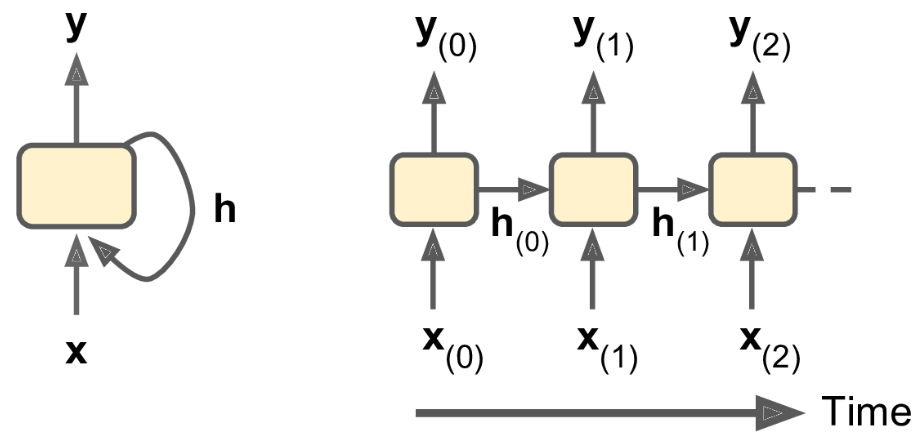
\includegraphics[width=.5\linewidth]{lstm/lstm_diagram.png}
    \caption{Block Diagram of a RNN}
    \label{fig:lstm_dia}
\end{figure}

\begin{comment}
Each neuron contains two sets of weights one which is used for the input and the other which is used on the feedback. Figure \cite{rnn_node} shows these weights as input weight (IW), and the delay weight (LW). The delay weight takes a delayed input delayed by block D. Block b is a bias weight which can be thought of as an offset which is applied to each neuron. The addition of these weights are added and input through an activation function in green. An output layer is typically (always) added to the output of the RNN. 
\begin{figure}[h]
    \centering
    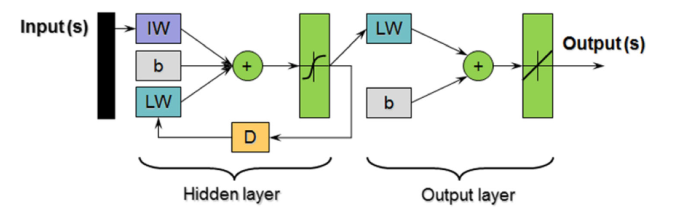
\includegraphics[width=.3\linewidth]{lstm/RNNnode.png}
    \caption{Block Diagram of a RNN}
    \label{fig:rnn_node}
\end{figure}
\end{comment} 

\subsection{Long Short Term Memory Networks}
LSTM networks are a particular subset of RNNs. The motivation and usage of an LSTM network are increased performance in long term dependencies in data at the cost of some additional computation power. An LSTM block takes an input $x_t$ and two states, the long term $c_{t-1}$ and short term $h_{t-1}$, which are used to determine the output state $h_t$ which is sent to the output layer. Three gates regulate information through the LSTM dropping or allowing memories based on pointwise operation controlled by weights $\sigma$. Essentially, the LSTM attempts to recognize important input. The Forget weight controlled by $f(t)$ regulates long term memories which should be erased. Input gate controlled by $i(t)$ adds memories to the long term memory. Output gate controlled by $o(t)$ allows long term states to be read by the output layer and passed on.  The governing equations for the LSTM block are shown below taken from \cite{hands_on_lstm}. $W_{xi}, W_{xf}, W_{xo}, W_{xg}$ are all neuron weights for the cell.  $W_{hi}, W_{hf}, W_{ho}, W_{hg}$ terms are weights from the previous short term state. Terms $b$ are bias terms or offsets. $Tanh$ functions can be changed and are the activation functions of the LSTM cell. The long term memory output $c_t$ of the cell is a function of the Forget gate and new inputs through the input gate. The short term memory and output y(t) is determined by the activation of the previous output modified by the activation of the long term memory. These gates can be seen in Figure \ref{fig:lstm_neuron}. Essentially, the LSTM network implements gates to increase the stability of learning both short term and long term memories in time series data by allowing and dropping certain memories from the cell. 

\noindent\begin{minipage}{.55\textwidth}
   \centering
   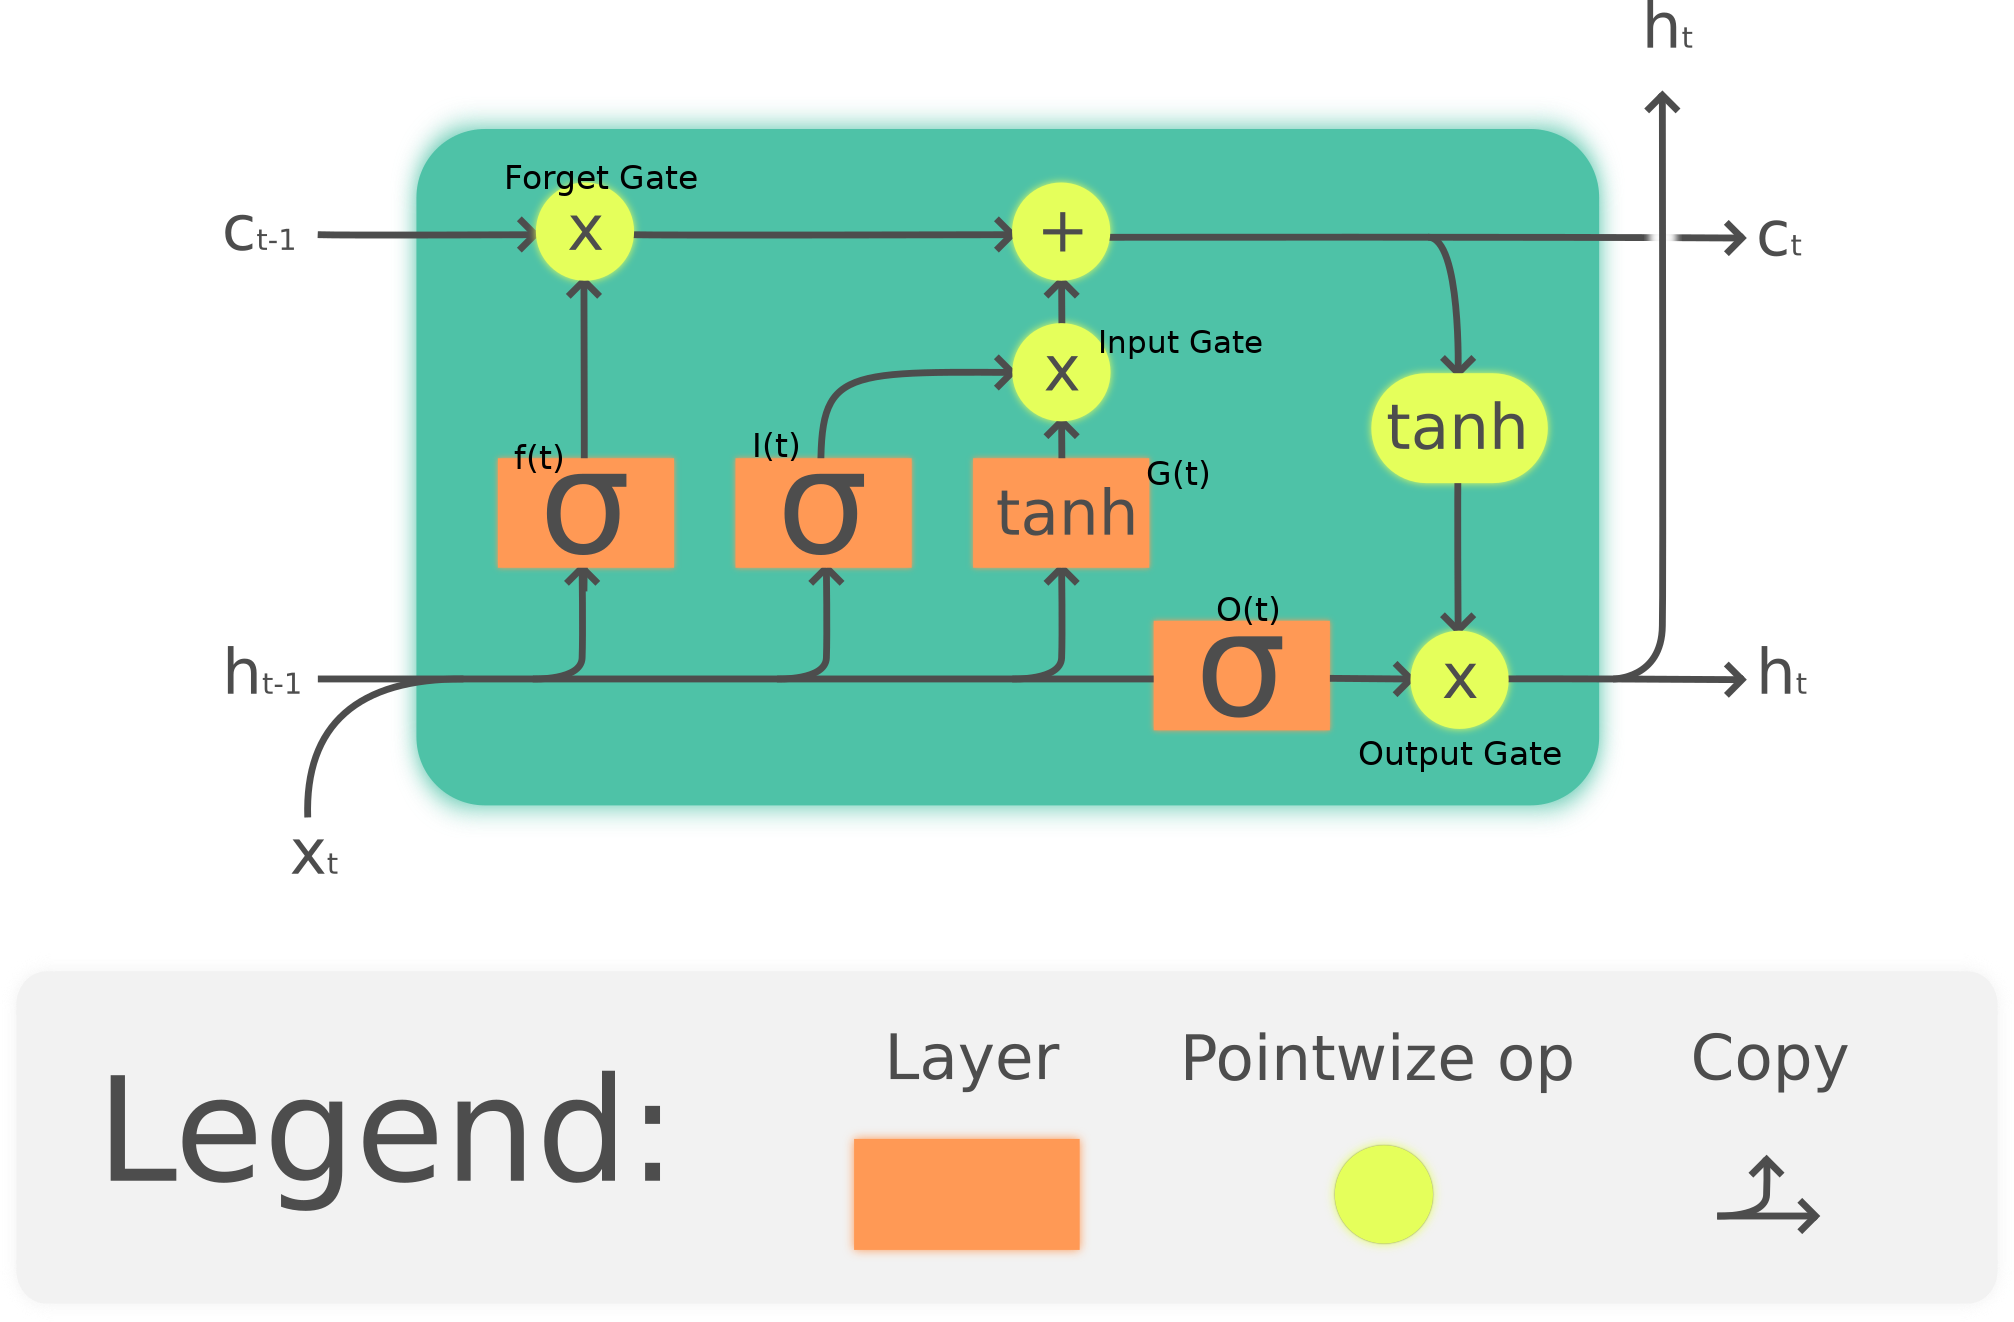
\includegraphics[width=\linewidth]{lstm/neuron_lstm.png}
   \captionof{figure}{Diagram of LSTM Neuron}
   \label{fig:lstm_neuron}
\end{minipage}
\begin{minipage}{.43\textwidth}
\begin{align}
        i(t) = \sigma(W_{xi}^Tx(t) + W_{hi}^Th(t-1) + b_i \\
        f(t) = \sigma(W_{xf}^Tx(t) + W_{hf}^Th(t-1) + b_f\\
        o(t) = \sigma(W_{xo}^Tx(t) + W_{ho}^Th(t-1) + b_o\\
        g(t) = tanh(W_{xg}^Tx(t) + W_{hg}^Th(t-1) + b_g\\
        c(t) = f(t) \bigotimes c(t-1) + i(t) \bigotimes g(t)\\
        y(t) = h(t) = o(t) \bigotimes tanh(c(t))
\end{align}
\end{minipage}

\subsection{LSTM Parameters}
Multiple different implementations were attempted to try and attain the lowest possible error. Two implementations were created, one using a simple method with a single feedback loop and another implementing data windowing. In addition to trying these two implementations, the parameters for each of these implementations were adjusted to attain the lowest possible loss on predicted data. 
\subsubsection{Simple LSTM}
 This method of LSTM network is the easiest implementation of an LSTM model which acts on time series data. The model acts on a single time step at a time, a diagram of the model is shown below in Figure \ref{fig:lstm_io}. The time of the run and the air data are fed into the neural network one time sample at a time. The output temperature data is fed back into the LSTM. The process repeats until all samples are consumed. The LSTM network is a collection of N neurons which are formed together to create a layer of LSTM cells which all receive the data and output the data. 
\begin{figure}[h]
    \centering
    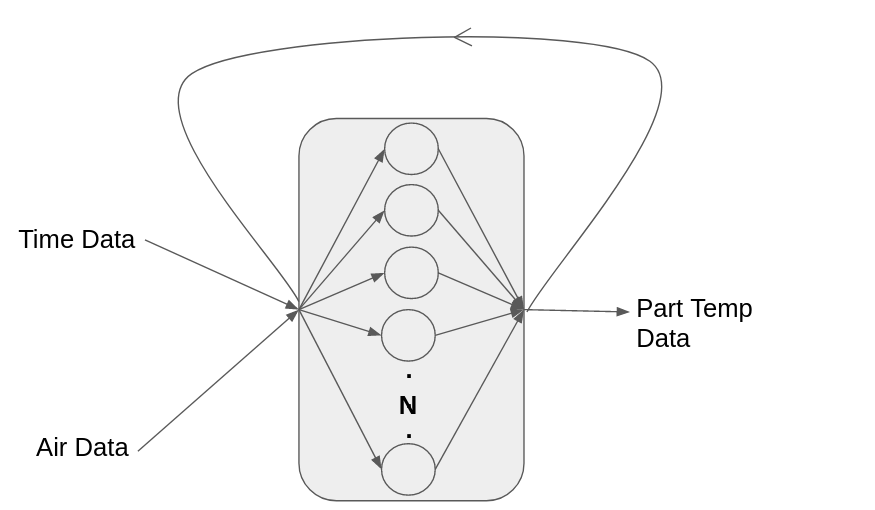
\includegraphics[width=.4\linewidth]{lstm/lstm_diagram_io.png}
    \caption{Input Output and feedback of LSTM layer}
    \label{fig:lstm_io}
\end{figure}
The time data and air temperature data is scaled to better accommodate the activation functions within the LSTM blocks which perform between the range of 0 and 1. The data varies in length but is set to 3600 in our LSTM networks to evaluate 60 minute runs with a single sample per second. In the case of the real data which is shorter than 3600 samples data is interpolated to increase its length. 
\subsubsection{Parameters} \label{lstmparameters}
The key parameters of the network include number of neurons, input dimension, dropout layer, and output layer. The LSTM layer consists of 25 neurons which take a three dimensional input array. Twenty-five neurons performed well on the data. A span between 10 to 50 resulted in fairly equal performance. The neurons are contained in a single hidden layer. Increasing the number of neurons has the possibility of over-fitting the data especially due to the low number of real runs that are available to train on. A higher number of neurons will also increase the training time. The network was set to ‘Stateful’ which means the network state is conserved through training batches. Through experimentation of different activation functions in the LSTM neuron, it was found that Softsign activation performs adequately. A Rectified Linear Unit (ReLU) activation also provided extremely similar performance. A dropout layer is added to the network to reduce over-fitting. The dropout layer thins the connections between neurons by randomly setting an input to a random neuron to zero depending on a certain rate \cite{dropout}. The rate is set to .0001 which is very low, as we are not overly concerned about over-fitting in our data set as the data set is so small it is almost unavoidable. An output layer is added to the LSTM network and adds a bias to the output of the LSTM layer and performs an activation function on it. A linear activation function was chosen for the output layer as it was found to be adequate, and changing to other activation functions produced worse predictions.
\subsubsection{Training}
The training optimizer used was Adam, it performed the best out of the ones tested including Adaptive gradient algorithm (AdaGrap) and Root Mean Square Propagation (RSMProp). Adam is the typical default optimizer used in machine learning algorithms \cite{learn_keras}. A slightly reduced learning rate of 0.0005 was used, which provided lower loss over the typical rate of .001. This is likely due to the network 'learning' the data more effectively, as opposed to over-fitting the data. The downside of reducing the learning rate is the network will take more iterations and more time to train. Each trial was trained on the LSTM network for a single epoch, then a new trial was selected from the training set and this was repeated until the loss was reduced adequately. The model is fit in batches meaning only portions of the data is given to the network at a time. Smaller batches can increase the stochasticity of the gradient descent during training  which can allow the algorithm to jump out of local minima and find the proper minimum for the network \cite{learn_keras}. A batch size of around 180 samples was found to be adequate. To calculate the loss, the mean-squared-error (MSE) loss function was used. This loss function is the standard and provides a harsh loss compared to other functions meaning small deviations will produce a higher relative loss. The loss function is shown in Equation \ref{lstm_loss}. It was found that moving to other loss functions always produced worse prediction capability. Usual training took up to 1000 epochs before the loss stopped being reduced on the validation set.
\begin{equation}\label{lstm_loss}
    \text{MSE} = \frac{1}{n}\sum^n_{i=1}(Y_i - \hat{Y}_i)^2
\end{equation}
 The loss during training of the network is shown in the figure below. It can be seen that the loss drops quickly at first and then slowly later, and the test loss is higher than the training loss. The network takes under 15 minutes to train on an Intel$^{\textregistered}$ Core$^{TM}$ I5-4760k 4core 3.4GHz Processor with time depending on the amount of training data used. 
\begin{figure}[h]
    \begin{subfigure}{.5\linewidth}.
        \centering
    	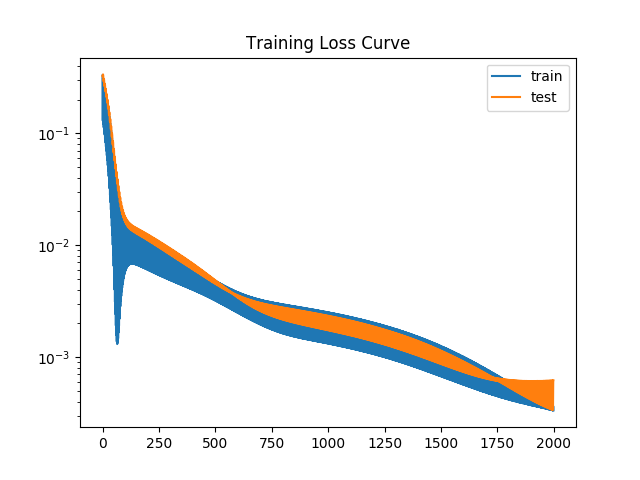
\includegraphics[width=\linewidth]{lstm/loss_f.png}
        \caption{Loss Curve 2000 epochs}
    \end{subfigure}
    \begin{subfigure}{.5\linewidth}.
        \centering
    	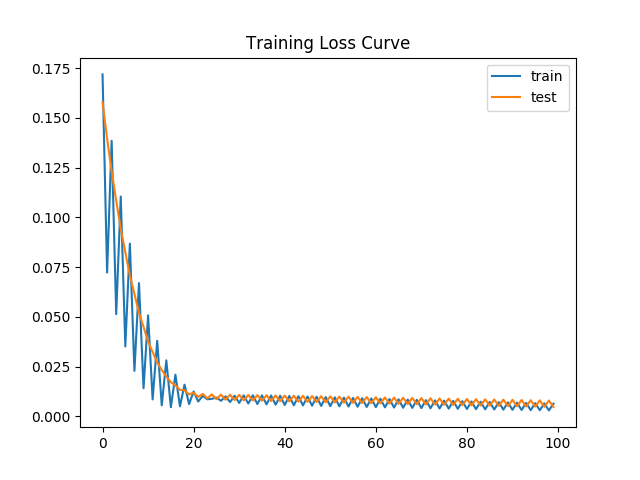
\includegraphics[width=\linewidth]{lstm/loss_2.png}
        \caption{Loss curve 100 epochs}
    \end{subfigure}\par\medskip
    \caption{Loss Graphs using MSE}
	\label{fig:loss}
\end{figure}

\subsubsection{Simple LSTM Simulated Data Performance}
The simulated data is a good case where there is a large pool of data and an interpolation is made on unknown data. The data is presented below in Figure \ref{fig:simulated_data_lstm}a. The machine learning algorithm shows a choppy output and the batch size can be seen where the machine learning algorithm was trained in batches. The error is low for all runs except for the first run shown in Figure \ref{fig:simulated_data_lstm}b but it can be seen that even this run is sufficient enough to make a prediction on soak time. It was also found that the performance could be vastly improved on simulated runs by scaling the temperature of trials using an individual max and min found from solely that trial. This would result in every temperature curve starting at 0 and ending at 1, and the rise of the part temperature would be extracted solely from the rise of the air temperature. Doing this kind of scaling would result in worse performance on real data as the air temperature does not exhibit a similar rise, so it was not used. 
\begin{figure}[ht]
    \begin{subfigure}{.5\linewidth}.
        \centering
    	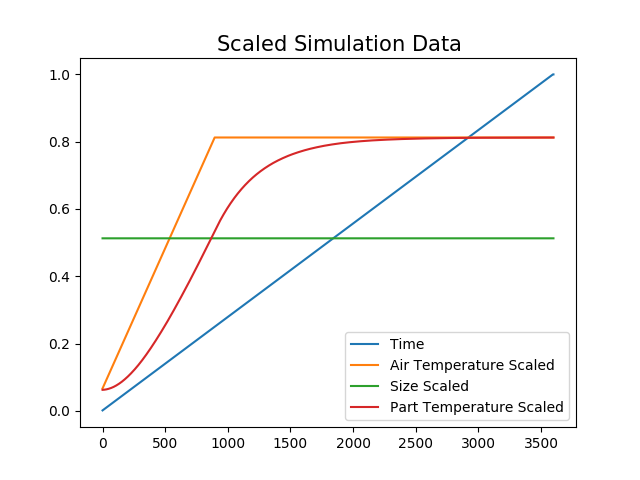
\includegraphics[width=\linewidth]{lstm/sime_data_scaling.png}
        \caption{Scaled Simulated data Input Features and truth}
    \end{subfigure}
    \begin{subfigure}{.5\linewidth}
    	\centering
    	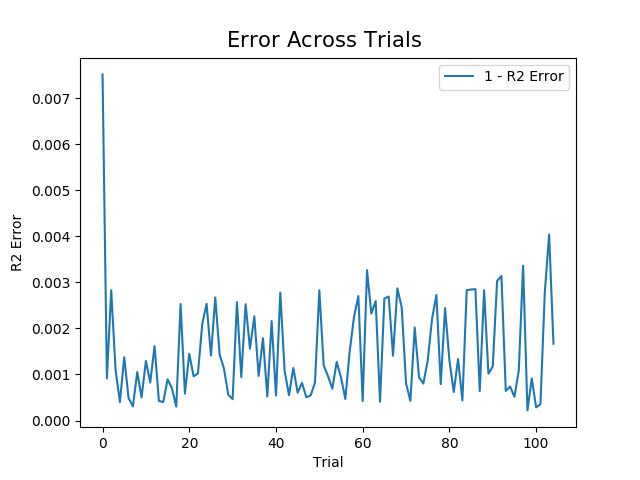
\includegraphics[width=\linewidth]{lstm/error.png}
    	\caption{Loss Across Runs R2 Error}	
    \end{subfigure}\par\medskip
    \begin{subfigure}{.5\linewidth}.
        \centering
    	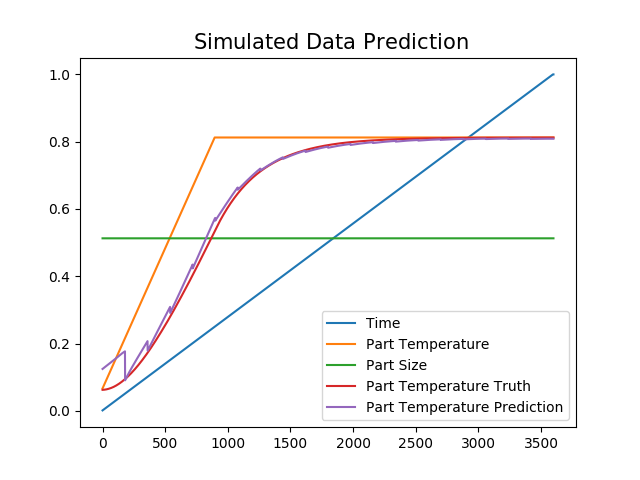
\includegraphics[width=\linewidth]{lstm/worst_sim_data.png}
        \caption{Highest Loss Run}
    \end{subfigure}
    \begin{subfigure}{.5\linewidth}
    	\centering
    	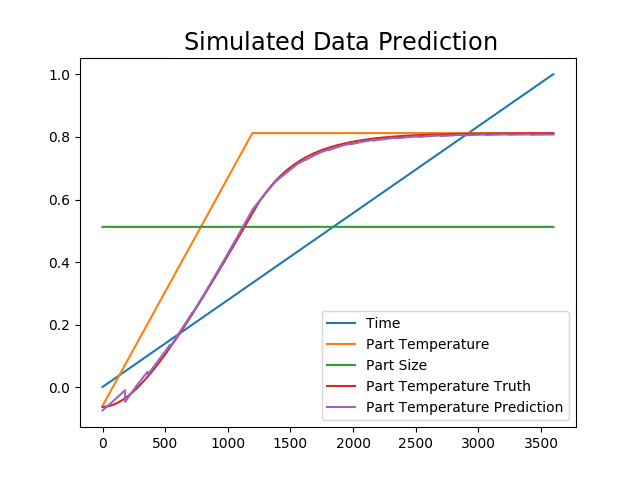
\includegraphics[width=\linewidth]{lstm/good_sim_data.png}
    	\caption{Average Loss Prediction}
    \end{subfigure}
    \caption{Simulated Data Information}
    \label{fig:simulated_data_lstm}
\end{figure}
\newpage
\subsubsection{Simple LSTM Real Data Performance} \label{simple_perf}
Real data was input two runs at a time and a prediction was then made on the third run. The summary of predictions is shown below in Figure \ref{fig:real_data_perf_lstm}. The predictions are better when stateful is set to false, most likely because the air data has a lower impact on the part temperature in the real data. The prediction of the 40$^\circ$C run by training on two 60$^\circ$C runs was poor due to the fact that no similar data was used to train and there was a limited amount of data to train on. 
\begin{figure}[ht]
    \begin{subfigure}{.34\linewidth}.
        \centering
    	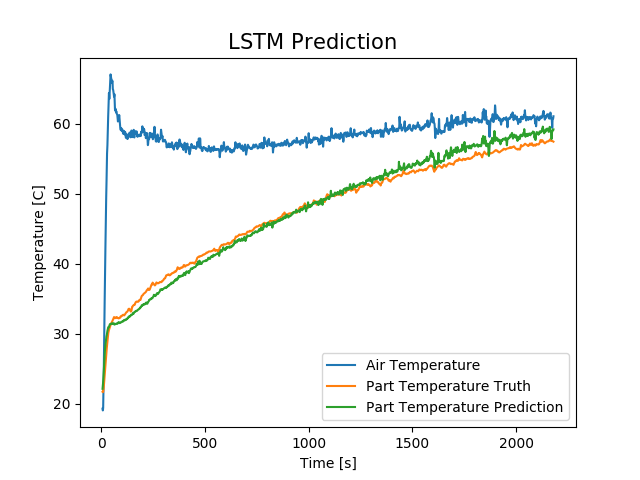
\includegraphics[width=\linewidth]{lstm/perf.png}
    \end{subfigure}
    \begin{subfigure}{.34\linewidth}
    	\centering
    	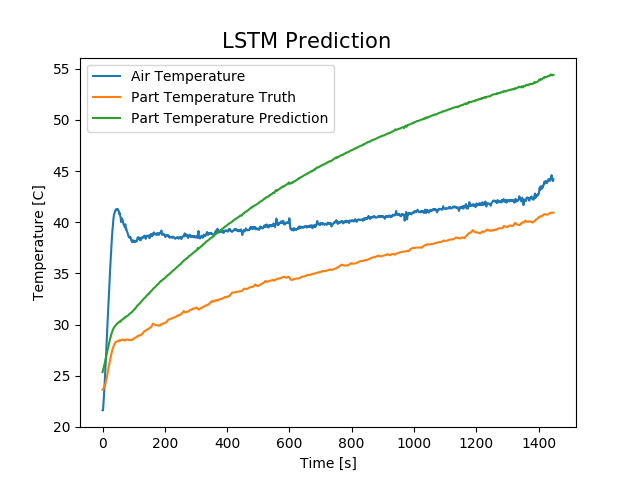
\includegraphics[width=\linewidth]{lstm/perf2.png}
    \end{subfigure}
    \begin{subfigure}{.34\linewidth}.
        \centering
    	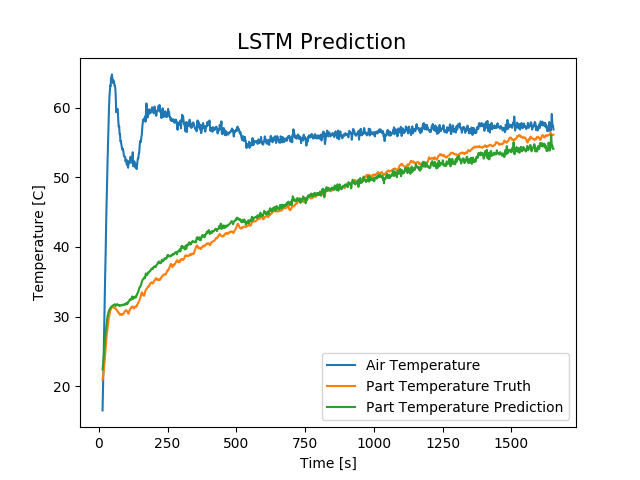
\includegraphics[width=\linewidth]{lstm/perf3.png}
    \end{subfigure}
    \caption{Real Data Predictions}
    \label{fig:real_data_perf_lstm}
\end{figure}
\newpage
\subsubsection{LSTM Windowed}
In an attempt to improve upon the simple LSTM model outlined above, another LSTM model was created using multiple time steps to make a decision. Unrolled, this model would be like the network below on the right. The network shares similar parameters to the other simple LSTM network. This network takes longer to train but can result in better predictions. The parameters used for the windowed method are the same as above and can be found in section \ref{lstmparameters}. 
\subsubsection{Windowed Data}
\begin{wrapfigure}{r}{0.5\textwidth}
  \vspace{-50pt}
  \begin{center}
    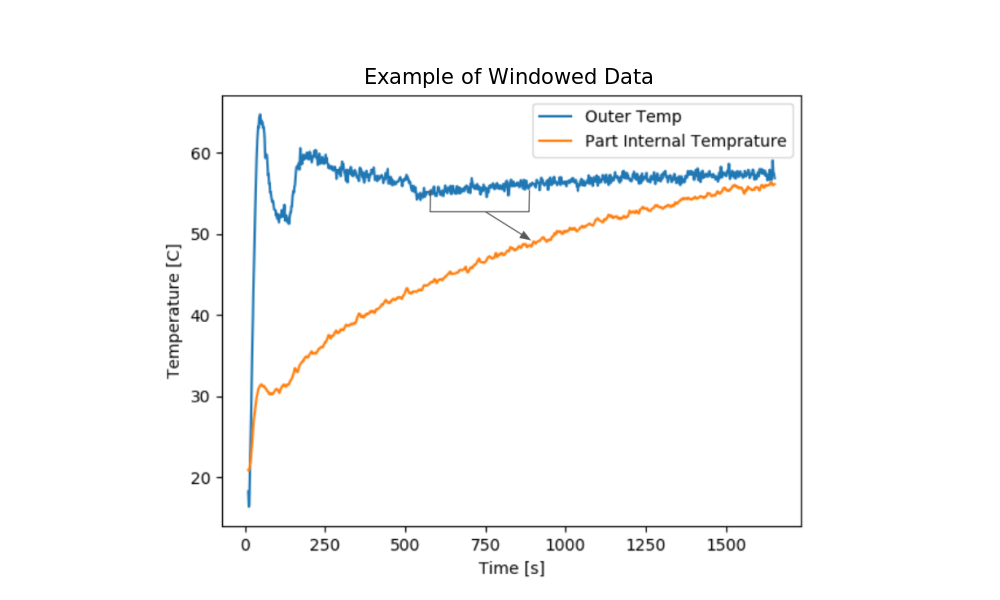
\includegraphics[width=0.6\textwidth]{lstm/window.png}
  \end{center}
  \vspace{-20pt}
  \caption{The window of data underlined which would be used to predict a single sample of part data which the arrow is pointing too}
  \label{fig:windowed}
  \vspace{-50pt}
\end{wrapfigure}
Windowed data is a way of organizing input features of the neural network to input samples and feed time data forward. The window implements a collection of data of past t-1 to t-N samples which are used to make a prediction on sample t. N can be any value, for our implementation a 50 sample window was chosen. An example of a window of data pointing at part temperature is shown in Figure \ref{fig:windowed} to the right, demonstrating what a window of data attempts to do. 

%\begin{figure}[h]
%    \centering
%    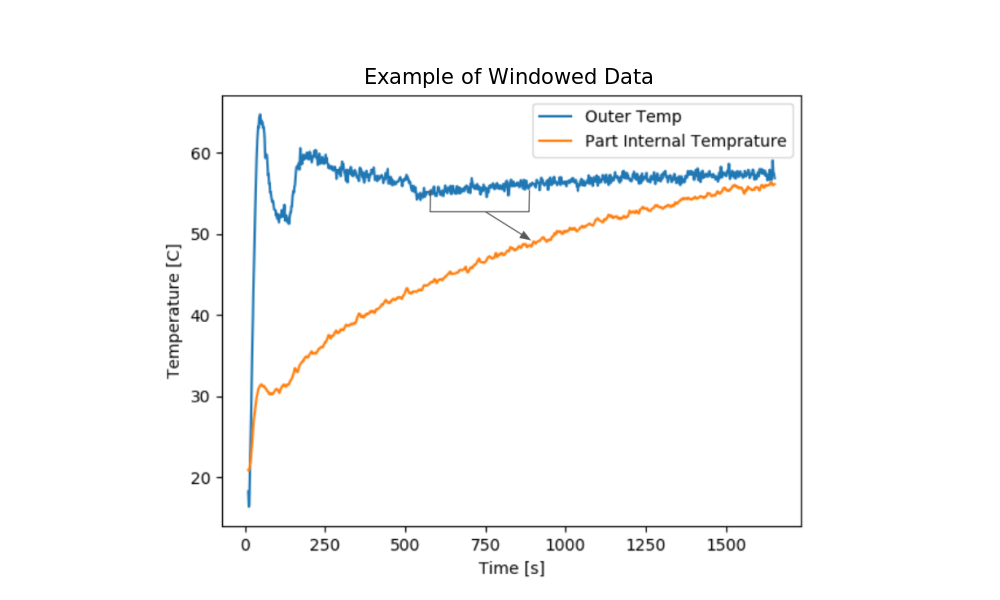
\includegraphics[width=.8\linewidth]{lstm/window.png}
%    \caption{Windowed Data Example}
%    \label{fig:windowed}
%\end{figure}
\newpage
\subsubsection{Windowed Method Prediction on Real Data}
The windowed method predicts slightly better than the simple method and is able to more closely fit data that it is trained on. It may also over-fit the data more. A dropout layer can help prevent over-fitting of the data although with this small of a data set to train on it makes minimal difference. From looking at the runs, it seems that the data is being learned more than overfit. This is exemplified by the dependency that part temperature has on the external air temperature shown by the hump from 500s-1000s in Figure \ref{fig:real_data_window_lstm1}. The end of the run matches closely with a percent error below 2\%, which is important for determining the soak time. Using Equation \ref{r2} the $R^2$ score was found for the first run to be 0.9824 and 0.9834 for the second run. Below in Figure \ref{fig:real_data_window_lstm1} \& \ref{fig:real_data_window_lstm2} the predictions are shown. The 40$^\circ$C run was not shown as it has a similar poor performance as the simple LSTM method shown above in Figure \ref{fig:real_data_perf_lstm} in section \ref{simple_perf}
\begin{figure}[ht]
    \begin{subfigure}{.5\linewidth}.
        \centering
    	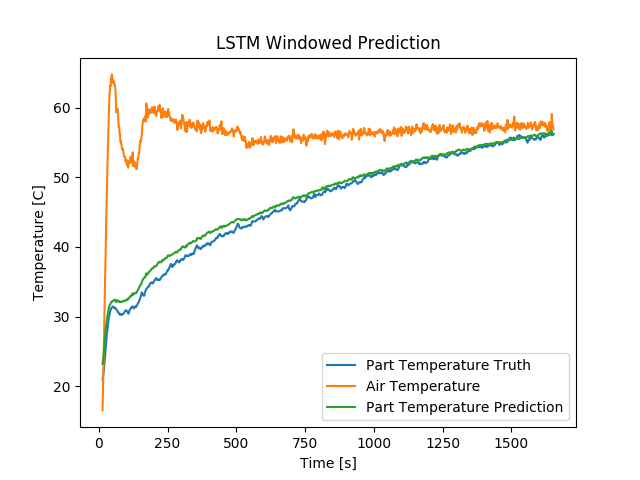
\includegraphics[width=\linewidth]{lstm/lstm_w_predict_april1.png}
    \end{subfigure}
    \begin{subfigure}{.5\linewidth}
    	\centering
    	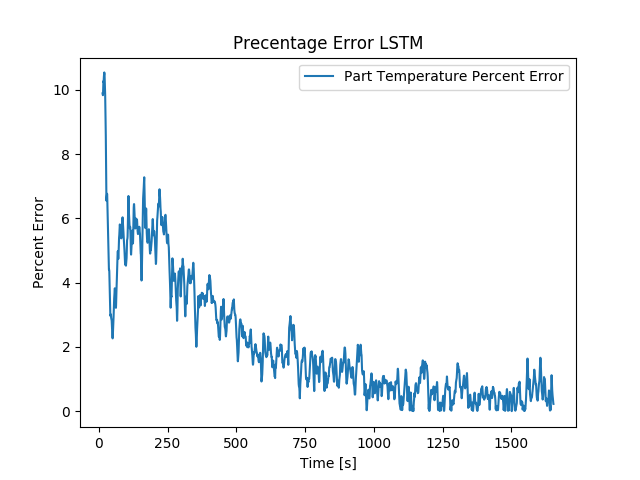
\includegraphics[width=\linewidth]{lstm/lstm_w_predict_april1_error.png}
    \end{subfigure}
    \caption{Real Data Predictions Windowed Data 1}
    \label{fig:real_data_window_lstm1}
\end{figure}
\begin{figure}[ht]
    \begin{subfigure}{.5\linewidth}.
        \centering
    	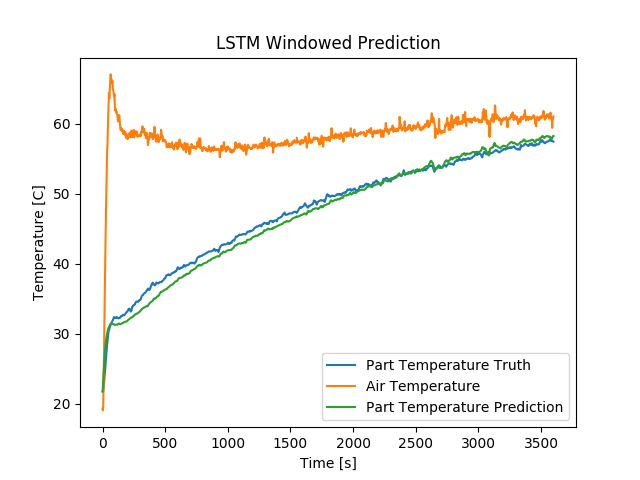
\includegraphics[width=\linewidth]{lstm/lstm_w_predict_april2.png}
    \end{subfigure}
    \begin{subfigure}{.5\linewidth}
    	\centering
    	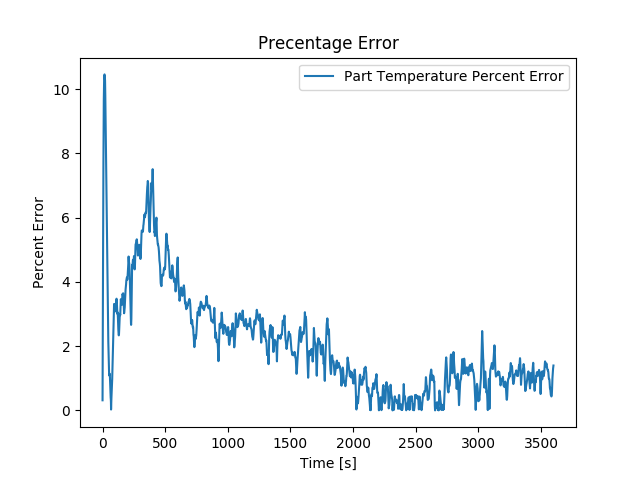
\includegraphics[width=\linewidth]{lstm/lstm_w_predict_april2_error.png}
    \end{subfigure}
    \caption{Real Data Predictions Windowed Data 2}
    \label{fig:real_data_window_lstm2}
\end{figure}
\newpage

\subsection{Soak Time Determination with LSTM}
The LSTM can also be used to make predictions from air data while the run is executing. This means that not all air temperature data is available so it is instead extrapolated to try and evaluate when the run should be finished. The simplest way to predict what the air temperature will do is to extrapolate by assuming it will hold the same temperature now until the end. Alternatives to this method include trying to do a polynomial regression or creating a neural network which predicts on air temperature. The extrapolation happens continually until a consensus on soak time can be made. \\\\
Below in Figure \ref{fig:live_predict} is an example of a prediction being made half way through one of the data sets. Here the soak time is set so that the part temperature should be within 5 percent of 55$^\circ$C so within about 53$^\circ$C and 57$^\circ$C. In Figure \ref{fig:live_predict} the prediction is being made at the blue vertical line using extrapolated data shown in red, the predicted soak time is shown in grey and the true prediction using part temperature truth is shown in black. It can be seen that the part temperature truth lost accuracy due to the extrapolation of air temperature. Click or double click on Figure \ref{fig:live_predict_gif} below to see a video of the live prediction being graphed out a step rate of roughly a prediction every five seconds.
%\href{movie.avi}{\includegraphics{video.avi}}
%\movie[options]{placeholder box}{video.avi}
%\href{movie.avi}{\movie[height = 0.1 \textwidth,width =\linewidth,showcontrols]{}{video.mpg}}
\begin{figure}[ht]
    \begin{subfigure}{.5\linewidth}.
        \centering
    	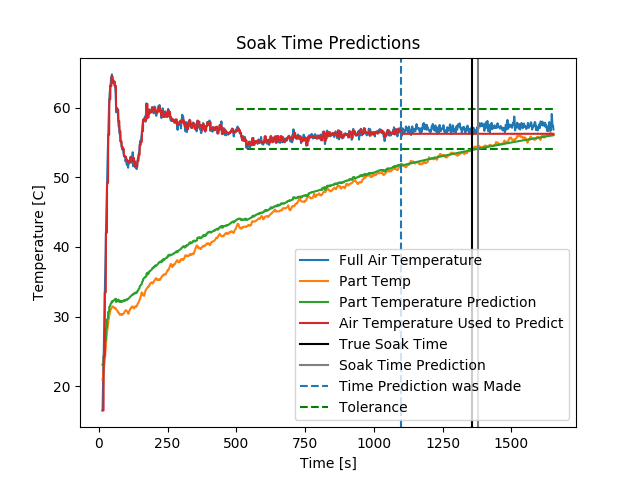
\includegraphics[width=\linewidth]{lstm/0plot_prediction_266.png}
    \end{subfigure}
    \begin{subfigure}{.5\linewidth}
    	\centering
    	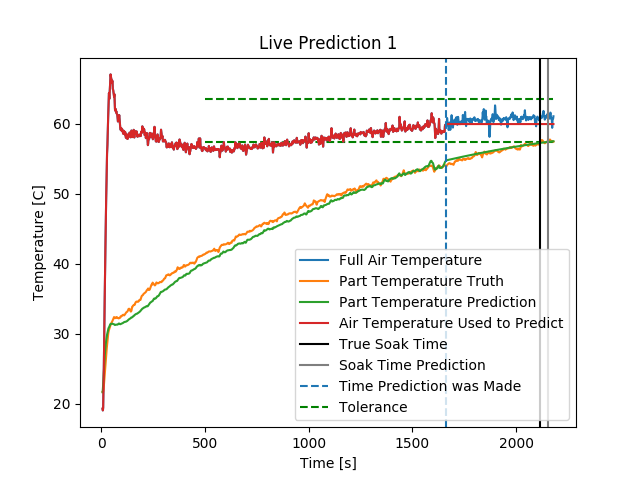
\includegraphics[width=\linewidth]{lstm/1plot_prediction_306.png}
    \end{subfigure}
    \caption{Live Predictions Windowed Data 1 \& 2}
    \label{fig:live_predict}
\end{figure}
\begin{figure}[h]
\centering
\begin{overpic}[width=0.5\textwidth]{lstm/0plot_prediction_266.png}
 \put (0,0){\includemovie[poster,text={\small(Click)}]{.5\textwidth}{6cm}{other/vid.mp4}}
\end{overpic}
\caption{Prediction video showing live prediction (double click, works in firefox), or follow the \href{https://www.youtube.com/watch?v=Oj7pGAFx5Rw&feature=youtu.be}{\textcolor{blue}{\underline{Link}}}}
\label{fig:live_predict_gif}
\end{figure}
\newpage
In Figure \ref{fig:live_predict_36} below, predictions were made on extrapolated data every five seconds. The plot in Figure \ref{fig:live_predict_36}a shows vertical lines in grey for every soak time that was predicted and a single black line for the true soak time. Figure \ref{fig:live_predict_36}b is a plot which shows the predicted soak time versus when that prediction was made. If the prediction is on the left half of the orange line, then that means it is predicting a soak time that is in the future. Once it starts predicting on a soak time in the past, the greatest confidence in accuracy has been achieved. One could then make a control decision to use the prediction that occurs as close as possible to the orange line to obtain the best accuracy. Using this control choice, a result was found where the estimated soak time of 1338.656 seconds versus the real soak time of 1356.877 seconds was found. This would result in a soak time about 20 seconds shorter than needed in a run which takes 22.3 minutes to complete. The other run estimated soak time as 2029.401 seconds when the true soak time was 2115.839 seconds and was 86 seconds off in a run that is 2179.91 seconds or 36.3 minutes long. It can be seen that as the run progresses and gets closer to the true soak time, its accuracy increases and converges to its final prediction. There is a small error in the soak time determined as the prediction is slightly different than the true part temperature curve.
\begin{figure}[ht]
    \begin{subfigure}{.5\linewidth}.
        \centering
    	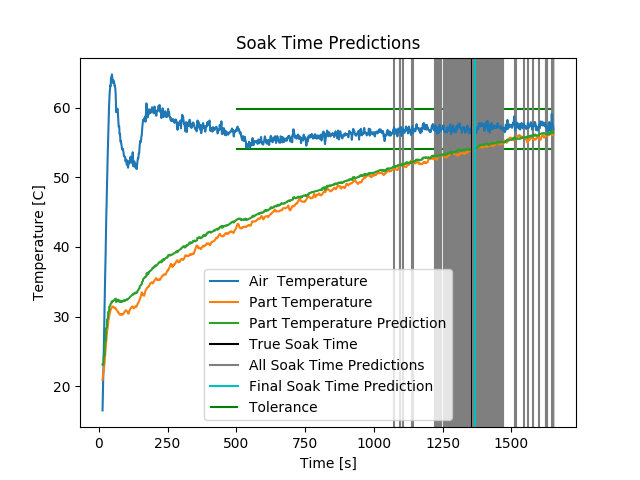
\includegraphics[width=0.9\linewidth]{lstm/soak_time_predictions.png}
        \caption{Soak Time Prediction Made every 5 seconds, Correct Prediction in Black, LSTM Predictions in Cyan/Grey}
    \end{subfigure}
    \begin{subfigure}{.5\linewidth}
    	\centering
    	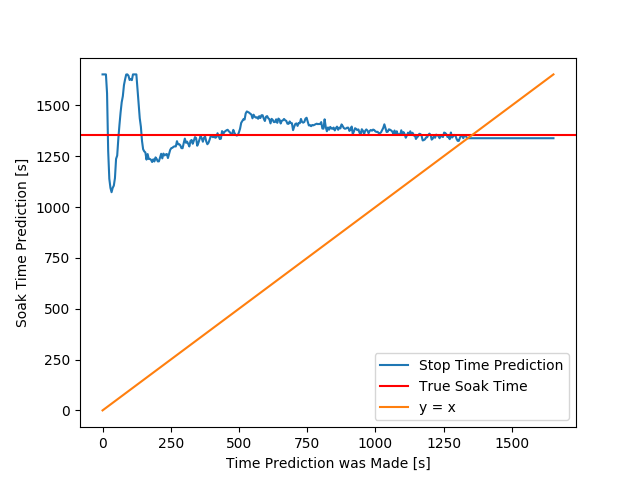
\includegraphics[width=0.9\linewidth]{lstm/soak_time_predictionsb.png}
        \caption{Soak Time Prediction and When it was made}
    \end{subfigure}
    \caption{Live Predictions}
    \label{fig:live_predict_36}
\end{figure}\clearpage
\subsection{Forward Prediction with LSTM}
It is also possible to train on every trial that is available in our data set then extrapolate the trend of air temperature to try to predict the future. This has use cases in seeing where the internal temperature is and how it will be in the future. This shows how soak time can be determined before it is reached allowing a control decision to be made. The simple LSTM’s prediction is shown below in Figure \ref{fig:Future_predct_win}. The trends are sensible except for the 40$^\circ$C run.
\begin{figure}[ht]
    \begin{subfigure}{.33\linewidth}.
        \centering
    	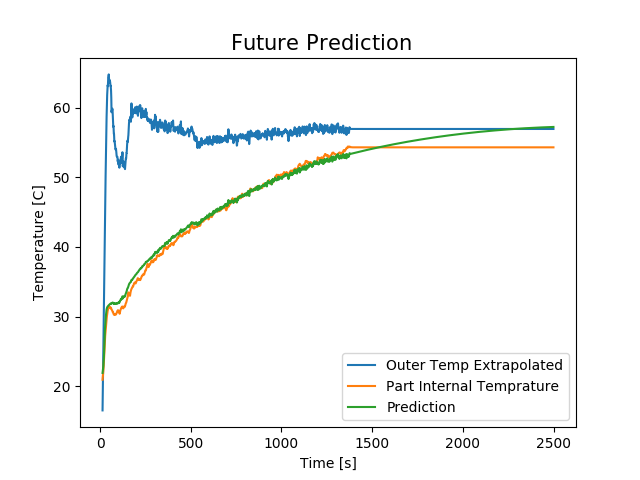
\includegraphics[width=\linewidth]{lstm/predict_f_w2.png}
    \end{subfigure}
    \begin{subfigure}{.34\linewidth}
    	\centering
    	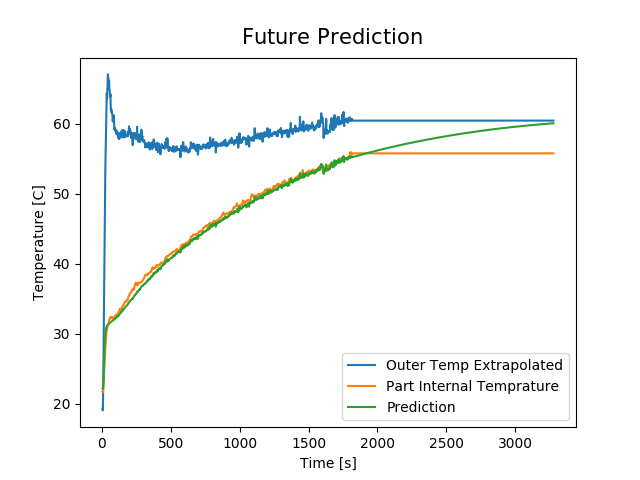
\includegraphics[width=\linewidth]{lstm/future_predict2.png}
    \end{subfigure}
    \begin{subfigure}{.33\linewidth}.
        \centering
    	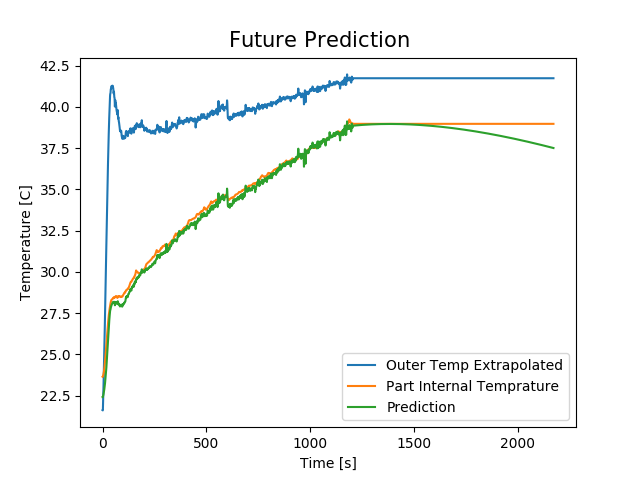
\includegraphics[width=\linewidth]{lstm/future_predict3.png}
    \end{subfigure}
    \caption{Future Data Predictions Simple Method}
    \label{fig:Future_predct_simple}
\end{figure}
\newline
Below in Figure \ref{fig:Future_predct_win} is the LSTM prediction into the future with the LSTM windowed method. As the air and part temperature converge the part temperature's slope does not decrease as expected. This would most likely result in an underestimate in soak time. Future predictions are an interesting look into how the LSTM believes the run will progress. It is hypothesized that with data that fully converges, these predictions would become more accurate. 
\begin{figure}[htb]
    \begin{subfigure}{.33\linewidth}.
        \centering
    	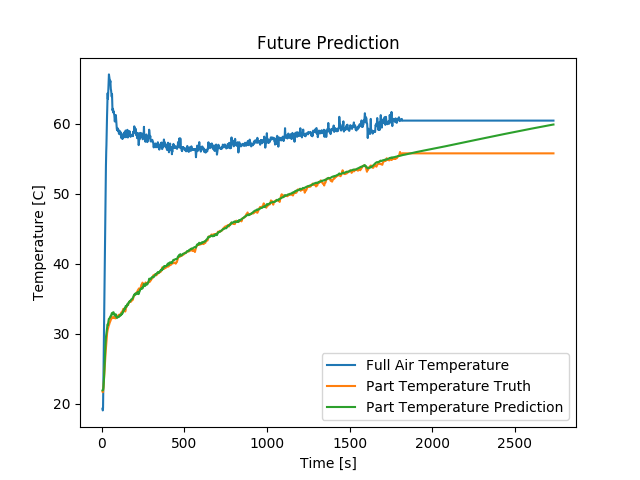
\includegraphics[width=\linewidth]{lstm/lstm_w_future1.png}
    \end{subfigure}
    \begin{subfigure}{.33\linewidth}
    	\centering
    	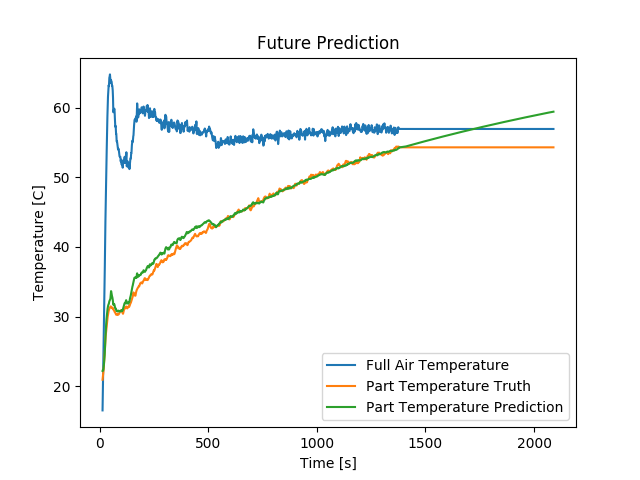
\includegraphics[width=\linewidth]{lstm/lstm_w_future2.png}
    \end{subfigure}
    \begin{subfigure}{.33\linewidth}.
        \centering
    	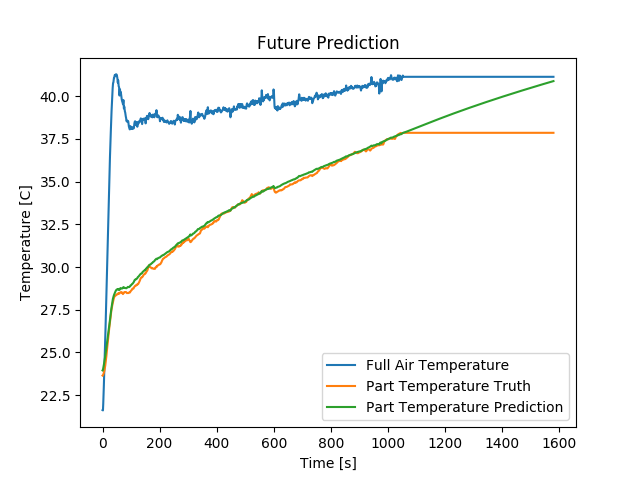
\includegraphics[width=\linewidth]{lstm/lstm_w_future3.png}
    \end{subfigure}
    \caption{Future Data Predictions Using Windowed Method}
    \label{fig:Future_predct_win}
\end{figure}
\clearpage
\subsection{Random Forests}
Random Forests operate on two main principles, decision trees and bagging. While according to \cite{RF}, Random Forests are popular mostly in classification tasks, it is a versatile algorithm that can be used to solve other tasks, such as regression. According to \cite{RF}, "A decision tree is a set of questions organized in a hierarchical manner and represented graphically as a tree". For each input, the decision tree asks successive questions about its known properties and splits into different paths. Depending on the path traversed through the tree, the questions asked will differ. Once the terminal leaf node (end of the path) is reached, the output is predicted.
\begin{figure}[!htb]
    \centering
    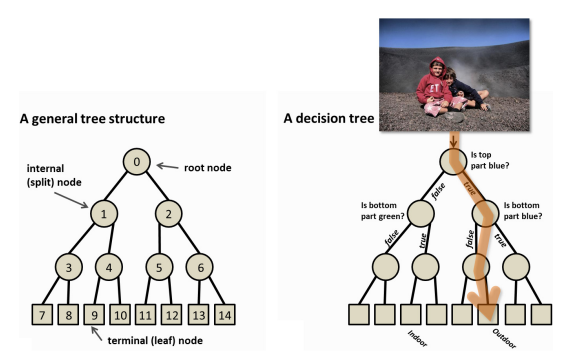
\includegraphics[width=0.5\linewidth]{other/decision_tree_RF.png}
    \caption{Diagram of Decision Tree Structure retrieved from \cite{RF}}
\end{figure}
\\\\To decide how paths are split, split functions based on metrics such as Information Gain, Gini Index, or Mean Squared Error are used. In Scikit-Learn's implementation of decision trees and Random Forests for regression, Mean Square Error is used by default (Eq. \ref{mse}) where $m$ represents a node, $R_{m}$ represents a region, and $N_{m}$ is the number of observations. Mean Absolute Error can also be selected as a split function for regression and is shown in Equation \ref{MAE}.
\begin{equation}
\bar{y}_{m} = \frac{1}{N_{m}}\sum_{i\in N_{m}}y_{i}    
\end{equation}

\begin{equation}
\label{mse}
    H(X_{m}) = \frac{1}{N_{m}} \sum_{i \in N_{m}}(y_{i} - \bar{y}_{m})^2
\end{equation}

\begin{equation}
\label{MAE}
    H(X_{m}) = \frac{1}{N_{m}}\sum_{i \in N_{m}}\mid y_{i} - y_{m}\mid
\end{equation}\\\\
Random Forests use the concept of bagging and an ensemble of decision trees to increase the performance over an individual decision tree. Bagging is a technique in which several weak learners, in this case decision trees, are trained on bootstrapped data sets with randomly selected features. Bootstrapped data sets for each decision tree are created by sampling the training data set with replacement, effectively resulting in different data sets. By randomly training decision trees on bootstrapped data sets, the correlation between each tree is reduced, improving generalization and robustness of the ensemble \cite{RF}.
\subsection{Random Forests Parameters \& Performance}
In this section, we analyze the parameters and performance of the Random Forests machine learning algorithm on the generated and real recorded data. 

\subsubsection{Parameters}
While there are various parameters such as the number of estimators, criterion, maximum depth of the tree, the minimum number of samples required to split a node, and the minimum number of samples required to be a leaf node, the parameters we used in our Random Forest model were left at the default settings. The reasoning behind this decision was because Random Forests are known to typically require minimal parameter tuning. Additionally, we did not have enough real-world data sets to cross-validate and tune the performance of our model before validating on a test set.

\subsubsection{Simulated Data}
Using simulated data, we can test the scenario in which we have a large pool of data and want to make a prediction on unseen data. The performance of Random Forests was evaluated with leave-one-out cross validation. In leave-one-out cross validation, given a pool of data sets, one data set is selected for testing while the remaining data sets are used as a training set. The score for each data set was then averaged which gives us our cross validation score. Scikit-Learn determines the performance of a model using $R^2$ which is determined by Equation \ref{r2} where $u$ is the residual sum of squares, $v$ is the total sum of squares, and $\bar{x}_{y_{true}}$ is the average of the true output labels. The score ranges from a value of 0-1 where 1 is the best possible score.

\begin{equation}
\label{r2}
    R^{2} = (1-\frac{u}{v}) \\
\end{equation}

\begin{equation}
        u = \sum (y_{true} - y_{pred})^{2}
\end{equation}

\begin{equation}
    v = \sum (y_{true} - \bar{x}_{y_{true}})^{2}
\end{equation}

In our testing, Random Forests performed quite well on simulated data and managed to get a cross validation score of 0.9986. Thus we can determine that on simulated data, Random Forests are a suitable method. An example of one of the tests in Figure \ref{RF_sim} shows that the ability of the Random Forest is near perfect. In this case, the percent error of a prediction at any given time constantly remains below 5\% as seen in Figure \ref{RF_sim_err}. The performance of the Random Forest appears to worsen as the slope of the internal temperature curve decreases, however once the internal temperature curve begins to flatten and the soak temperature is met, the Random Forest predictions stabilize.

\begin{figure}[ht]
    \begin{subfigure}{.5\linewidth}.
        \centering
    	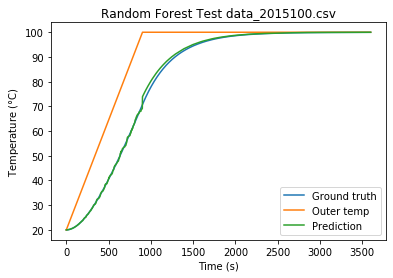
\includegraphics[width=\linewidth]{other/RF_prediction_simulated.png}
        \caption{Prediction with Random Forests}
        \label{RF_sim}
    \end{subfigure}
    \begin{subfigure}{.5\linewidth}
    	\centering
    	\includegraphics[width=\linewidth]{other/RF_error_simulated.png}
        \caption{Percent Error}
        \label{RF_sim_err}
    \end{subfigure}
    \caption{Simulated Data Performance using Random Forests}
\end{figure}

\subsubsection{Real Data}
When testing on our real-world data, we once again used leave-one-out testing. In this case since the amount of data we have is minimal, we will look at the results of each test individually. As our data was initially very noisy, we first ran our data through a Kalman filter before training the Random Forest. Looking at the results of max60run1 in Figure \ref{rf601} and \ref{rf601err}, we can see that the Random Forest has decent performance with an $R^2$ score of 0.9608 and typically has a \% error of less than 5\%.

\begin{figure}[ht]
    \begin{subfigure}{.5\linewidth}.
        \centering
    	\includegraphics[width=\linewidth]{other/RF_prediction_real.png}
        \caption{Prediction with Random Forests}
        \label{rf601}
    \end{subfigure}
    \begin{subfigure}{.5\linewidth}
    	\centering
    	\includegraphics[width=\linewidth]{other/RF_error_real.png}
        \caption{Percent Error}
        \label{rf601err}
    \end{subfigure}
    \caption{Real Data Performance using Random Forests - Testing max60run1}
\end{figure}

For max60run2 in Figure \ref{rf602} and \ref{rf602err}, the performance is initially quite good before diverging around the 350 second mark. Around the 700 second mark, the predictions became very unstable before stabilizing when the part gets close to the designated soak temperature. The poor performance in this case can likely be attributed to over-fitting due to a lack of variety in data. 

\begin{figure}[ht]
    \begin{subfigure}{.5\linewidth}.
        \centering
    	\includegraphics[width=\linewidth]{other/RF_prediction_real2.png}
        \caption{Prediction with Random Forests}
        \label{rf602}
    \end{subfigure}
    \begin{subfigure}{.5\linewidth}
    	\centering
    	\includegraphics[width=\linewidth]{other/RF_error_real2.png}
        \caption{Percent Error}
        \label{rf602err}
    \end{subfigure}
    \caption{Real Data Performance using Random Forests - Testing max60run2}
\end{figure}

On the max40 run, in Figure \ref{rf40} and \ref{rf40err}, the performance as expected is incredibly poor. This poor performance is expected as the Random Forest was not trained on a temperature curve with a maximum temperature of 40$^\circ$C. The typical scenario that should be expected is to train the model on a range of temperature curves where the test data set will fall in between.

\begin{figure}[ht]
    \begin{subfigure}{.5\linewidth}.
        \centering
    	\includegraphics[width=\linewidth]{other/RF_prediction_real3.png}
        \caption{Prediction with Random Forests}
        \label{rf40}
    \end{subfigure}
    \begin{subfigure}{.5\linewidth}
    	\centering
    	\includegraphics[width=\linewidth]{other/RF_error_real3.png}
        \caption{Percent Error}
        \label{rf40err}
    \end{subfigure}
    \caption{Real Data Performance using Random Forests - Testing max40}
\end{figure}